\chapter{基于图过滤的程序依赖图表征学习}
\label{chap:PDG}
本章主要对本文提出的基于图过滤的程序依赖图表征学习方法进行详细介绍,首先介绍其基本思想,其次阐述其具体方法设计与实现,最后进行实验验证。

\section{研究动机}
\label{sec:PDGMotivation}

程序依赖图PDG是代码的一种图形表示,所含结构信息最多,能够表示程序的控制依赖,数据依赖等关系,是一种带有标记的有向多重图。程序依赖图PDG结点代表语句,边代表依赖关系,依赖关系包括数据依赖和控制依赖。基于图的代码表征方法首先使用代码分析工具构建包含代码语法结构、调用关系、数据流等信息的程序依赖图,然后通过子图匹配的方法,将PDG图中的控制流和数据流编码为一个紧凑的语义特征矩阵,其中每个元素都是一个高维的稀疏二值特征向量。通过将代码表示为图的形式使得模型能够更好地理解代码中不同部分之间的依赖关系,更适合研究代码内的丰富语义信息。

基于图的代码表征方法存在两种主要限制:

(1)规模开销较高:基于图的表征学习方法通常需要构建代码的结构图或控制流图作为分析的基础,对于具有复杂控制流或数据流的代码片段,构建准确的图表示是一个不小的挑战。特别地,当代码片段中具有循环、递归或异常处理机制时,图的构建过程更加困难。这些复杂结构不仅增加图构建的复杂性,还有可能导致图表示的精度下降;即使在成功生成图之后,图表征学习方法的计算成本也很高。例如,对图进行子图同构等操作时,往往需要借助复杂的图算法来实现,并将生成的程序依赖图两两匹配,对于包含$n$个代码片段的数据集,需要进行$n^2$次匹配检测。而其中包含大量无用的匹配,会浪费大量的时间和计算资源。这些算法不仅计算成本大,而且随着代码库规模的扩大,处理时间也会显著增加,导致开销高。

(2)对代码修改的敏感性:在实际开发过程中,代码通常会经过各种微小的更改,例如变量名更改、代码格式化、添加或删除注释等,这些修改可能会导致图的表示发生显著变化。具体来说,当代码中的变量名被更改时,图的节点和边可能会受到影响,因为变量名通常作为图中的一个重要特征被考虑在内。同样,代码格式的调整,如缩进、换行或空格的变化,虽然不影响代码的逻辑功能,但也可能导致图的拓扑结构发生变化。此外,添加或删除注释虽然对代码的执行没有影响,但在构建代码图时,这些注释也可能被当作图的一部分,从而影响到图的表示。因此,基于图的克隆检测方法可能无法准确地检测出这些轻微修改过的克隆代码。更进一步,随着代码库的不断增长和变化,基于图的克隆检测方法可能需要不断地更新和调整以适应新的代码结构。这意味着方法的实现和维护成本可能会相对较高,因为开发者需要定期更新和调整方法以适应代码的变化。这种持续的更新和调整不仅增加了工作负担,还可能影响到方法的长期有效性。

因此,针对上述问题,本文提出了一种基于图过滤的程序依赖图表征学习方法,该方法通过预处理图过滤,减少候选PDG对集合的规模。

\section{PDG表征方法方法设计}
\label{sec:PDG}
本节将介绍基于图过滤的程序依赖图表征学习方法设计与实现,首先介绍该方法的整体框架,并从图过滤、程旭依赖图表征学习两方面介绍具体设计。 

\subsection{框架概述}
\label{subsec:PDGOverview}
本文提出的基于图过滤的程序依赖图表征学习方法整体框架如图\ref{fig:pdgframework}所示。该框架的输入是代码片段对应的程序依赖图,输出是对应的语义特征向量,主要包括图过滤、图表征两个阶段。

\begin{figure}[H]
  \centering
  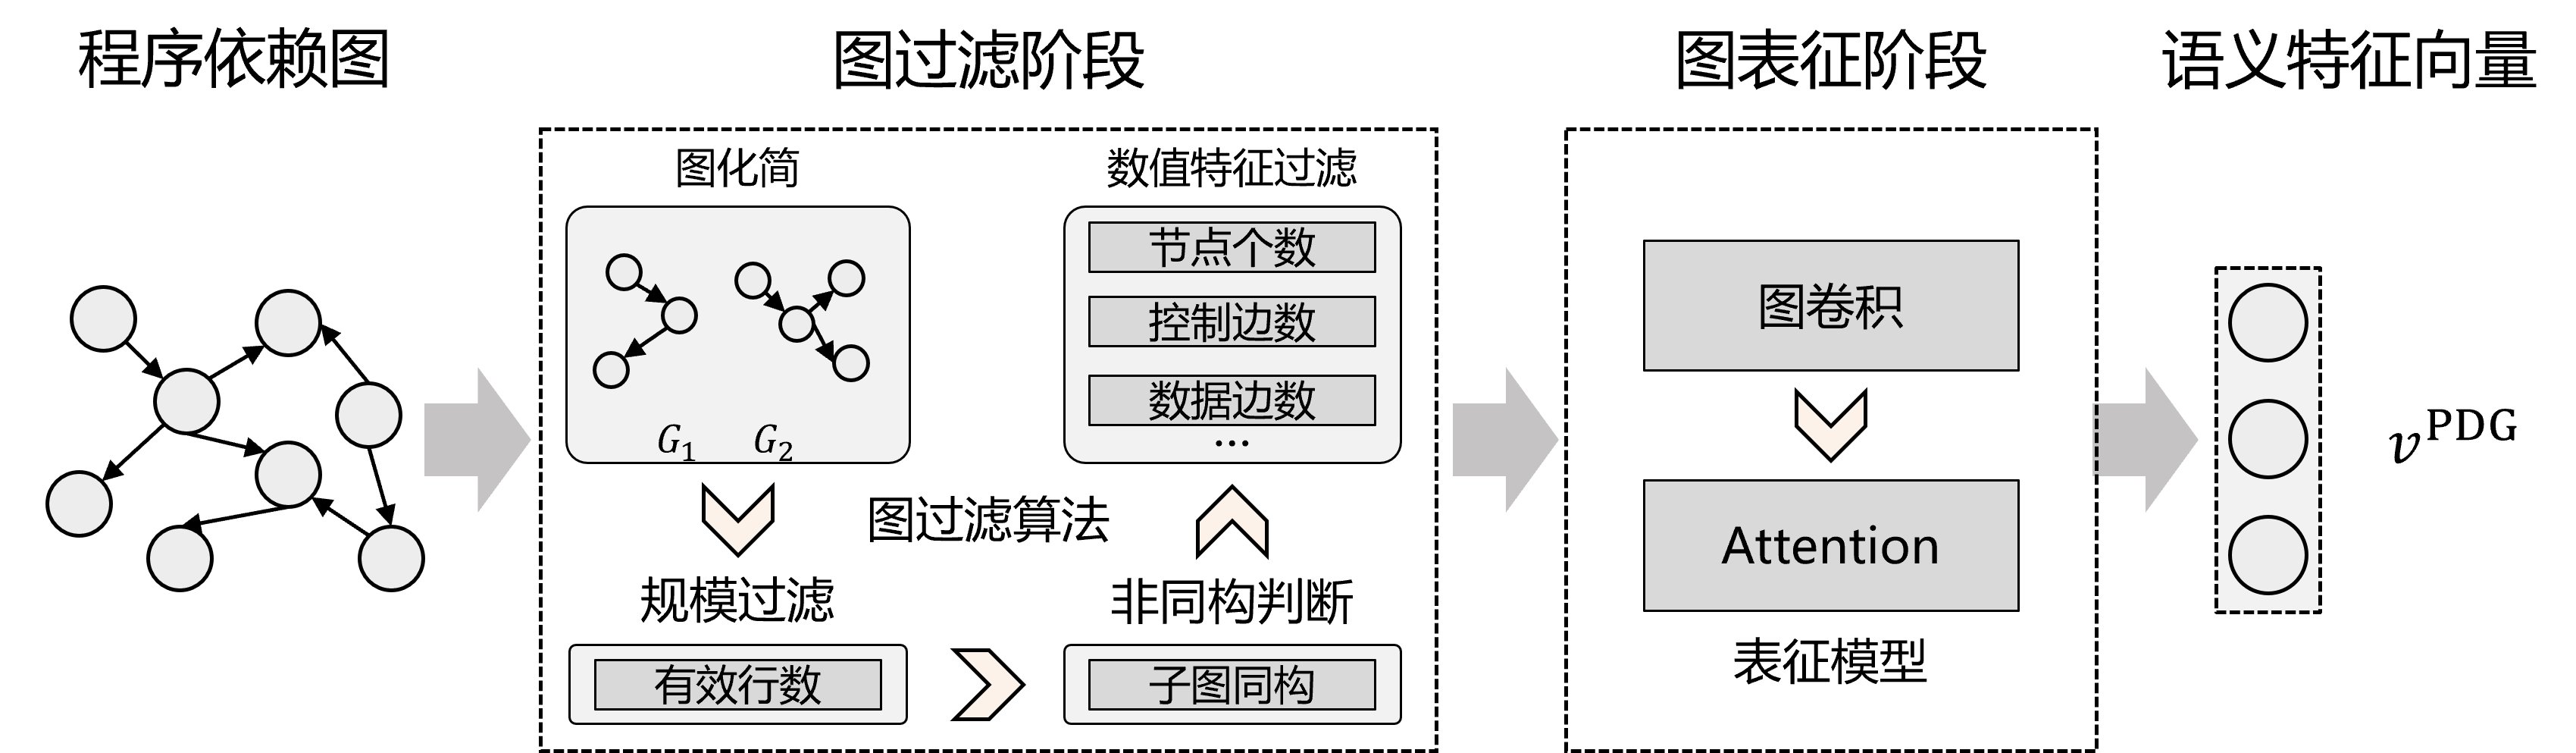
\includegraphics[width=0.95\textwidth]{figures/pdgframework.png}
  \caption{基于图过滤的程序依赖图表征学习框架}\label{fig:pdgframework}
\end{figure}

首先,图过滤阶段以代码片段对应的程序依赖图作为训练数据,设计一个基于候选程序依赖图对的图过滤算法,通过减少候选图对的规模,提高后续模型的训练能力。需要注意的是,为了更好地减少图规模,本文设计了一些有效的过滤策略,通过对PDG的边进行约简、对PDG对集合进行过滤的方式,只保留克隆可能性较大地候选PDG对,从而有效地加速检测过程,减少后续模型输入规模。

其次,图代码表征阶段以过滤后的程序依赖图作为训练数据,构建一个图表征模型。该模型的输入是程序依赖图,输出为一个固定长度的密集向量用来表示代码的语义特征。需要注意的是,本文选用的图卷积神经网络,主要包含两个部分:图卷积部分和自注意力机制部分,前者主要目的是通过在图上的卷积操作来捕捉节点的特征以及节点之间的关系。后者的主要目的是总结图节点特征,并将每个代码片段缩减为一个单一的密集向量。

在上述框架中,本文的创新点主要体现在图过滤阶段的图过滤算法、图代码表征阶段的模型设计两方面,下面将围绕这两个创新点来阐述本文的方法。


\subsection{图过滤设计}
\label{subsec:PDGPreModel}

本文使用代码分析工具Joern生成程序依赖图。其中,Joern通过静态分析源代码,生成关键的图结构信息,反映代码中的依赖关系和函数调用层次,同时Joern提供查询和可视化功能,用户可以通过命令将分析结果导出为多种格式,从而更好地理解代码的逻辑和流程。使用Joern工具,生成代码片段\ref{fig:code1}对应的程序依赖图,并导出DOT文件如\ref{fig:pdgshili1}所示,使用开源图形可视化工具Graphviz对DOT文件进行转化,可以得到如\ref{fig:pdgshili2}的图形。

\begin{figure}[H]
  \centering
  \subfigure[代码片段1对应的PDG DOT格式]{   %第一张子图
      \centering    %子图居中
      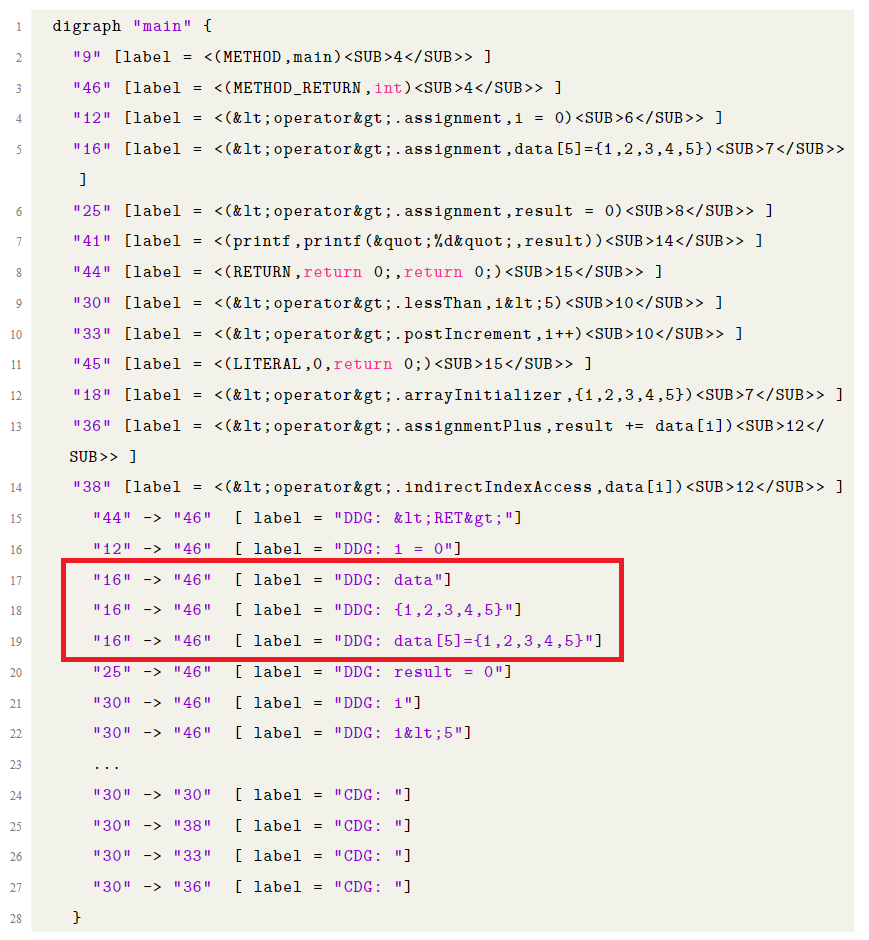
\includegraphics[width=0.4\textwidth]{figures/pdgshili}  
      \label{fig:pdgshili1} %引用标签
  }
  \subfigure[代码片段1对应的PDG可视化]{ %第二张子图
      \centering    %子图居中
      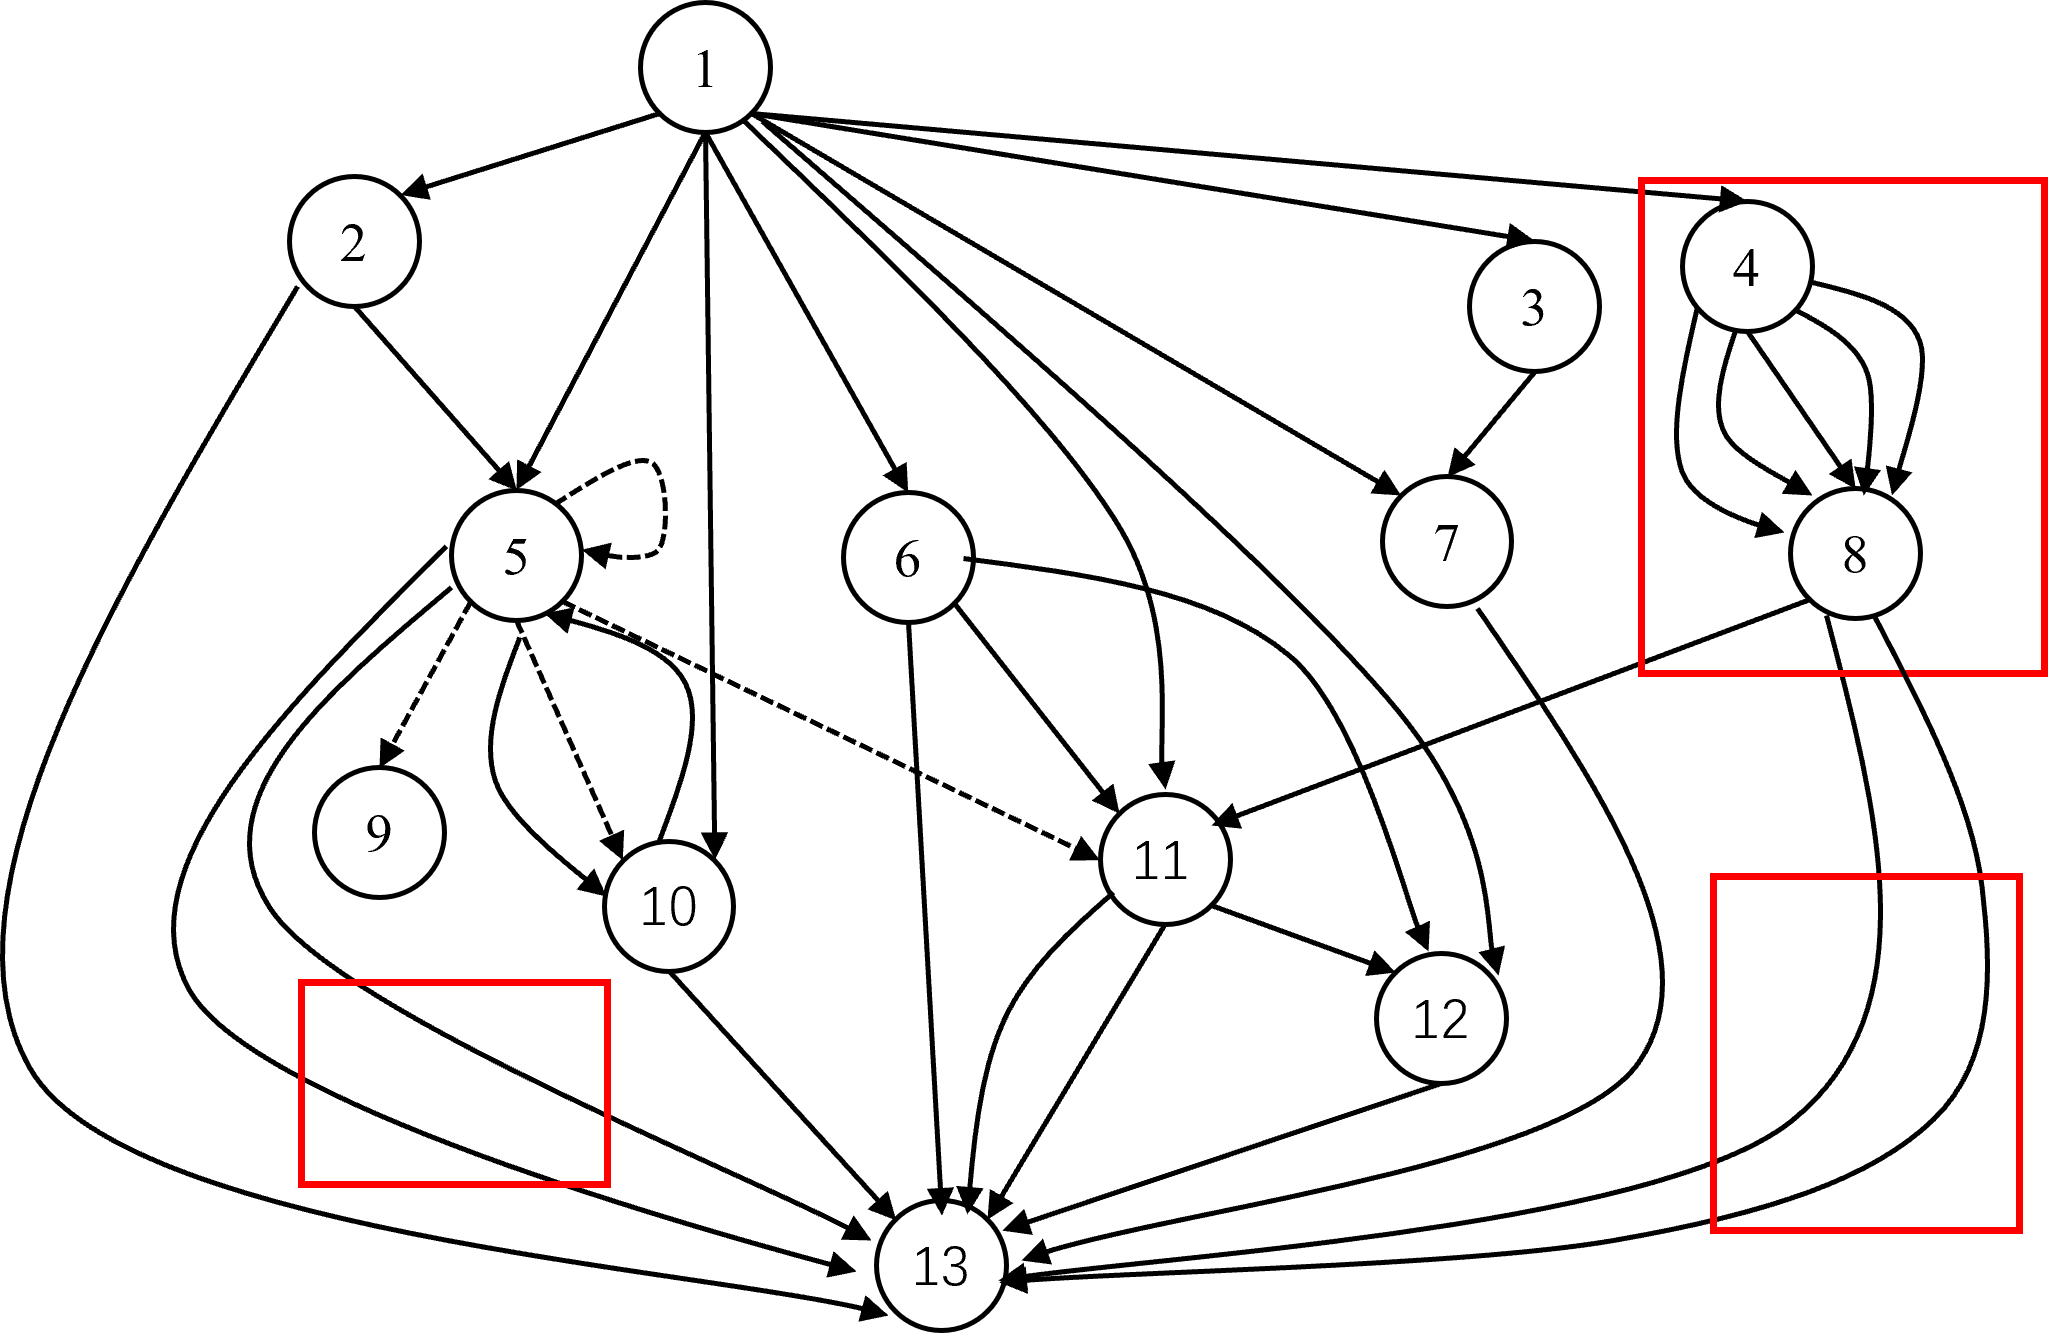
\includegraphics[width=0.5\textwidth]{figures/pdgshili2}
      \label{fig:pdgshili2} %引用标签
  }
  \caption{程序依赖图DOT文件示例}
  \label{fig:pdgshili}
\end{figure}
% \lstset{language=C}
% \begin{lstlisting}
%   digraph "main" {  
%     "9" [label = <(METHOD,main)<SUB>4</SUB>> ]
%     "46" [label = <(METHOD_RETURN,int)<SUB>4</SUB>> ]
%     "12" [label = <(&lt;operator&gt;.assignment,i = 0)<SUB>6</SUB>> ]
%     "16" [label = <(&lt;operator&gt;.assignment,data[5]={1,2,3,4,5})<SUB>7</SUB>> ]
%     "25" [label = <(&lt;operator&gt;.assignment,result = 0)<SUB>8</SUB>> ]
%     "41" [label = <(printf,printf(&quot;%d&quot;,result))<SUB>14</SUB>> ]
%     "44" [label = <(RETURN,return 0;,return 0;)<SUB>15</SUB>> ]
%     "30" [label = <(&lt;operator&gt;.lessThan,i&lt;5)<SUB>10</SUB>> ]
%     "33" [label = <(&lt;operator&gt;.postIncrement,i++)<SUB>10</SUB>> ]
%     "45" [label = <(LITERAL,0,return 0;)<SUB>15</SUB>> ]
%     "18" [label = <(&lt;operator&gt;.arrayInitializer,{1,2,3,4,5})<SUB>7</SUB>> ]
%     "36" [label = <(&lt;operator&gt;.assignmentPlus,result += data[i])<SUB>12</SUB>> ]
%     "38" [label = <(&lt;operator&gt;.indirectIndexAccess,data[i])<SUB>12</SUB>> ]
%       "44" -> "46"  [ label = "DDG: &lt;RET&gt;"] 
%       "12" -> "46"  [ label = "DDG: i = 0"] 
%       "16" -> "46"  [ label = "DDG: data"] 
%       "16" -> "46"  [ label = "DDG: {1,2,3,4,5}"] 
%       "16" -> "46"  [ label = "DDG: data[5]={1,2,3,4,5}"] 
%       "25" -> "46"  [ label = "DDG: result = 0"] 
%       "30" -> "46"  [ label = "DDG: i"] 
%       "30" -> "46"  [ label = "DDG: i&lt;5"] 
%       ...
%       "30" -> "30"  [ label = "CDG: "] 
%       "30" -> "38"  [ label = "CDG: "] 
%       "30" -> "33"  [ label = "CDG: "] 
%       "30" -> "36"  [ label = "CDG: "] 
%     }
% \end{lstlisting}

%\notag \right.\\\left.

分析上图\ref{fig:pdgshili1},程序依赖图DOT文件的描述包含两个部分:使用\textquotedbl number \textquotedbl [label =  <\(function,name\)> ]来描述PDG点的特征,包括节点编号、节点的标签,其中标签内还包括源代码语句中的变量名称、变量属性等信息。使用\textquotedbl number \textquotedbl $\to$ \textquotedbl number \textquotedbl [label = \textquotedbl CDG/DDG:data \textquotedbl ]来描述PDG边的特征,包括边的起始点编号、边的终点标号、边代表的依赖关系(控制依赖用CDG表示、数据依赖用DDG表示)。使用开源图形可视化工具Graphviz得到的图\ref{fig:pdgshili2}中包含13个顶点,用实线箭头表示数据依赖边,虚线箭头表示控制依赖边。通过DOT描述语言存储生成的PDG能够很好的表现出代码片段的语法信息,表示出不同的节点和边的各种特征和属性,为下一步的过滤算法打好基础。

如果代码片段功能复杂,那么对应的程序依赖图规模也会很大,同时包含很多冗余边。例如上图\ref{fig:pdgshili2}中红框中的边,它们起始节点、终止节点均相同。右上角的红框对应\ref{fig:pdgshili1}中的data数组,数组内包含5个元素,对应含有5条边。实际上,这些边只有数值不同,属性相同,因此需要进行适当的优化来使得程序程序依赖图的结构精简,又不会丢失语义信息。

针对上述问题,本文设计了一种基于候选图对集合的图过滤算法,算法的伪代码如\ref{alg3}所示。该算法有多个输入:候选程序依赖图集合$G$、PDG有效行数阈值$L$、程序依赖图对规模比率$T$,输出为:经过过滤后的PDG对集合$R$,初该算法分为四个步骤:PDG图结构化简、规模过滤、非同构判断、数值特征过滤,每个步骤的作用如下:

\begin{algorithm}[ht]  
	\renewcommand{\algorithmicrequire}{\textbf{Input:}}
	\renewcommand{\algorithmicensure}{\textbf{Output:}}
	\caption{Graph filter algorithm $\left(filter\_PDG\right)$}  
	\label{alg3}
	\begin{algorithmic}[1]
    \Require PDG pairs:$G$
    \Require The threshold:$L$
    \Require The threshold of PDG pair's scale ratio:$T$
    \Require The threshold of CV's string numberical similarity:$G_s$
		\Ensure Candidate PDG pairs:$R$
    \State initialization
		\For{each PDG paris $G_1,G_2$  $in$ $G$}
      \State deleteSelfLoops($G_1$)
      \State deleteSelfLoops($G_2$) \Comment{step1:PDG图结构化简}
      \If {sizeof($G_1$) < L or sizeof($G_2$) < L}
        \State PDG pair($G_1,G_2$) is filtered \Comment{step2:规模过滤}
      \Else
        \If {min($G_1,G_2$) / max($G_1,G_2$) < T}
          \If{there is subgraph between ($G_1,G_2$ )} \Comment{step3:非同构判断}
            \State R $\leftarrow$ R $\cup \left(G_1,G_2\right)$ 
          \Else
            \State PDG pair($G_1,G_2$ ) is filtered
          \EndIf
        \Else
          \If {number similarity of $G_1,G_2$ > $G_s$} \Comment{step4:数值特征过滤}
            \State R $\leftarrow$ R $\cup \left(G_1,G_2\right)$
          \Else
            \State PDG pair($G_1,G_2$ ) is filtered
          \EndIf
        \EndIf
      \EndIf 
    \EndFor \\
    \Return $R$
	\end{algorithmic}
\end{algorithm}

(1)PDG图结构化简:首先对候选程序依赖图集合中的图进行化简,对起始节点、终止节点均相同的边进行化简,仅保留一条边,从而减少图的大小以便后续图匹配操作。下图\ref{fig:pdgshili3}是化简后的结果。

\begin{figure}[H]
  \centering
  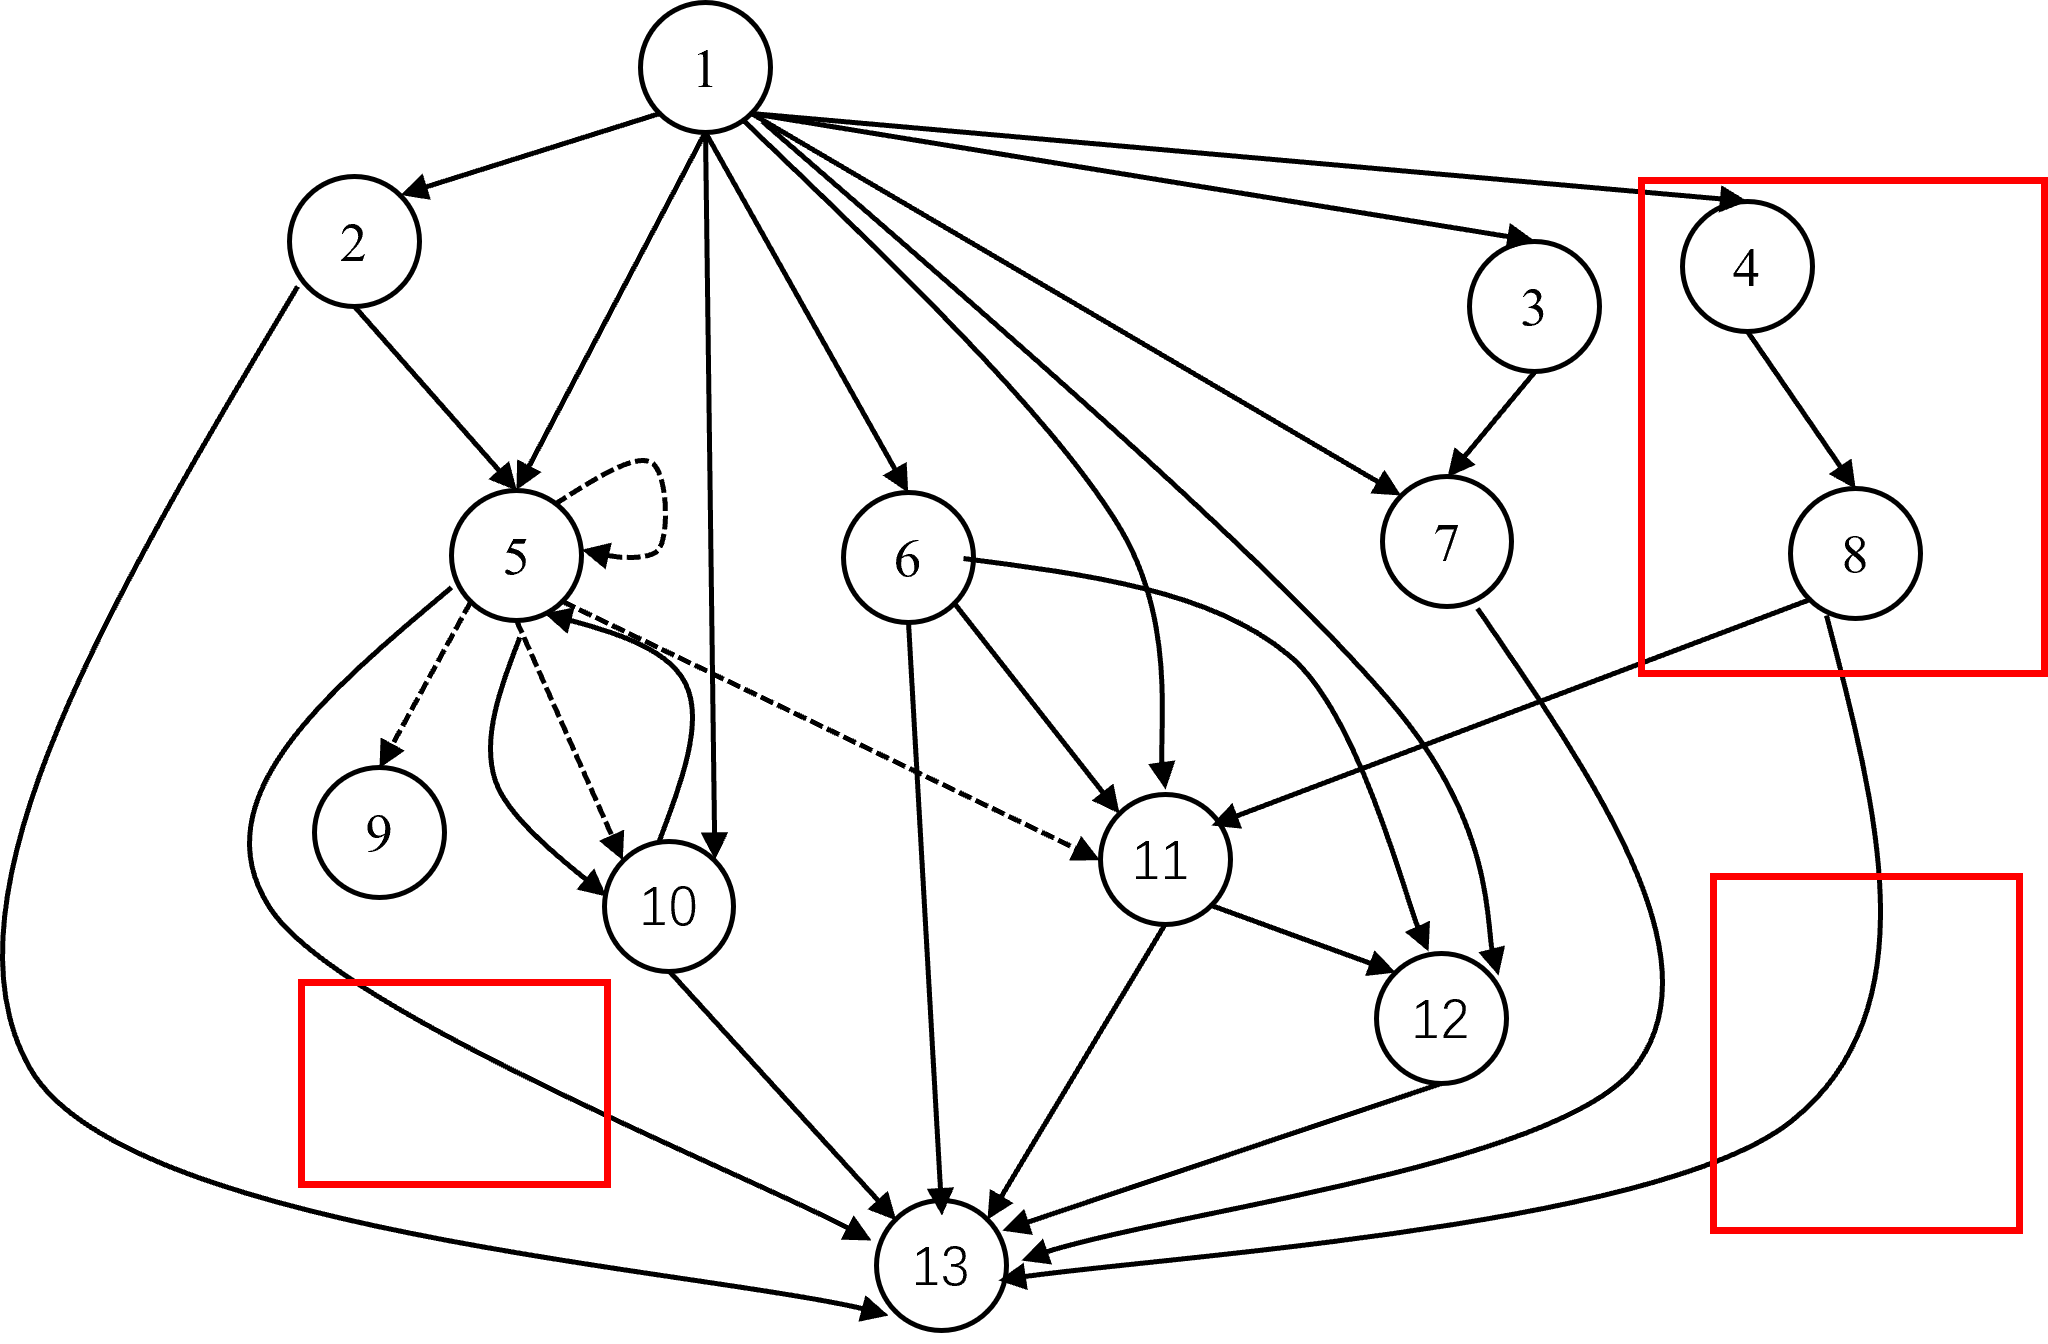
\includegraphics[width=0.55\textwidth]{figures/pdgshili3.png}
  \caption{代码片段1经过图结构化简后的图}\label{fig:pdgshili3}
\end{figure}

(2)规模过滤:其次对图的规模进行判断,针对代码克隆检测,有研究证明,有效行数小于6行的克隆程序本身并没有任何意义,并且会被绝大多数的代码克隆检测工具忽略.因为小于6行有效行的函数多为空函数,没有太大的参考意义。因此,本文也设置一个阈值,如果PDG1和PDG2中有任意一个PDG的有效行数小于阈值,那么就需要过滤掉这对PDG。

(3)非同构判断:接着对PDG对中是否存在子图同构进行判断。假设一对PDG对中,规模较大的图为$G_1$,规模较小的图为$G_2$,根据子图同构的概念,只要$G_1$和$G_2$满足以下两个条件之一:
\begin{equation}\label{e5.1}
  \begin{split}
    max(O(G_1)) < max(O(G_2)) \\
    min(I(G_1)) < min(I(G_2))
  \end{split}
\end{equation}

那么这两个图就不可能存在子图同构关系。其中$O(G)$表示程序依赖图的节点出度,$I(G)$表示程序依赖图的节点入度。如果这对PDG不存在子图同构,但节点总数相差很大,那么就需要过滤掉这对PDG。

(4)数值特征过滤:最后通过收集PDG的简单特征来过滤掉明显不可能为克隆的PDG对。具体的,根据PDG的节点个数、控制边数、执行边数、数据边数、声明节点数、函数调用数、传入参数、传出参数等代表特征进行过滤,这些特征包含了代码一定的语义和语法信息。通过过滤掉差异很大的PDG对,从而减少候选PDG对集合的规模。


\subsection{程序依赖图表征学习设计}
\label{subsec:PDGModel}

(1)结构设计

为了提高程序依赖图维度代码表征能力,本文选取图卷积网络对上述得到程序依赖图进行建模。具体的模型设计如图\ref{fig:pdgmodel}所示。该模型主要包括输入层、多层卷积层、自注意力层、输出层。
\begin{figure}[H]
  \centering
  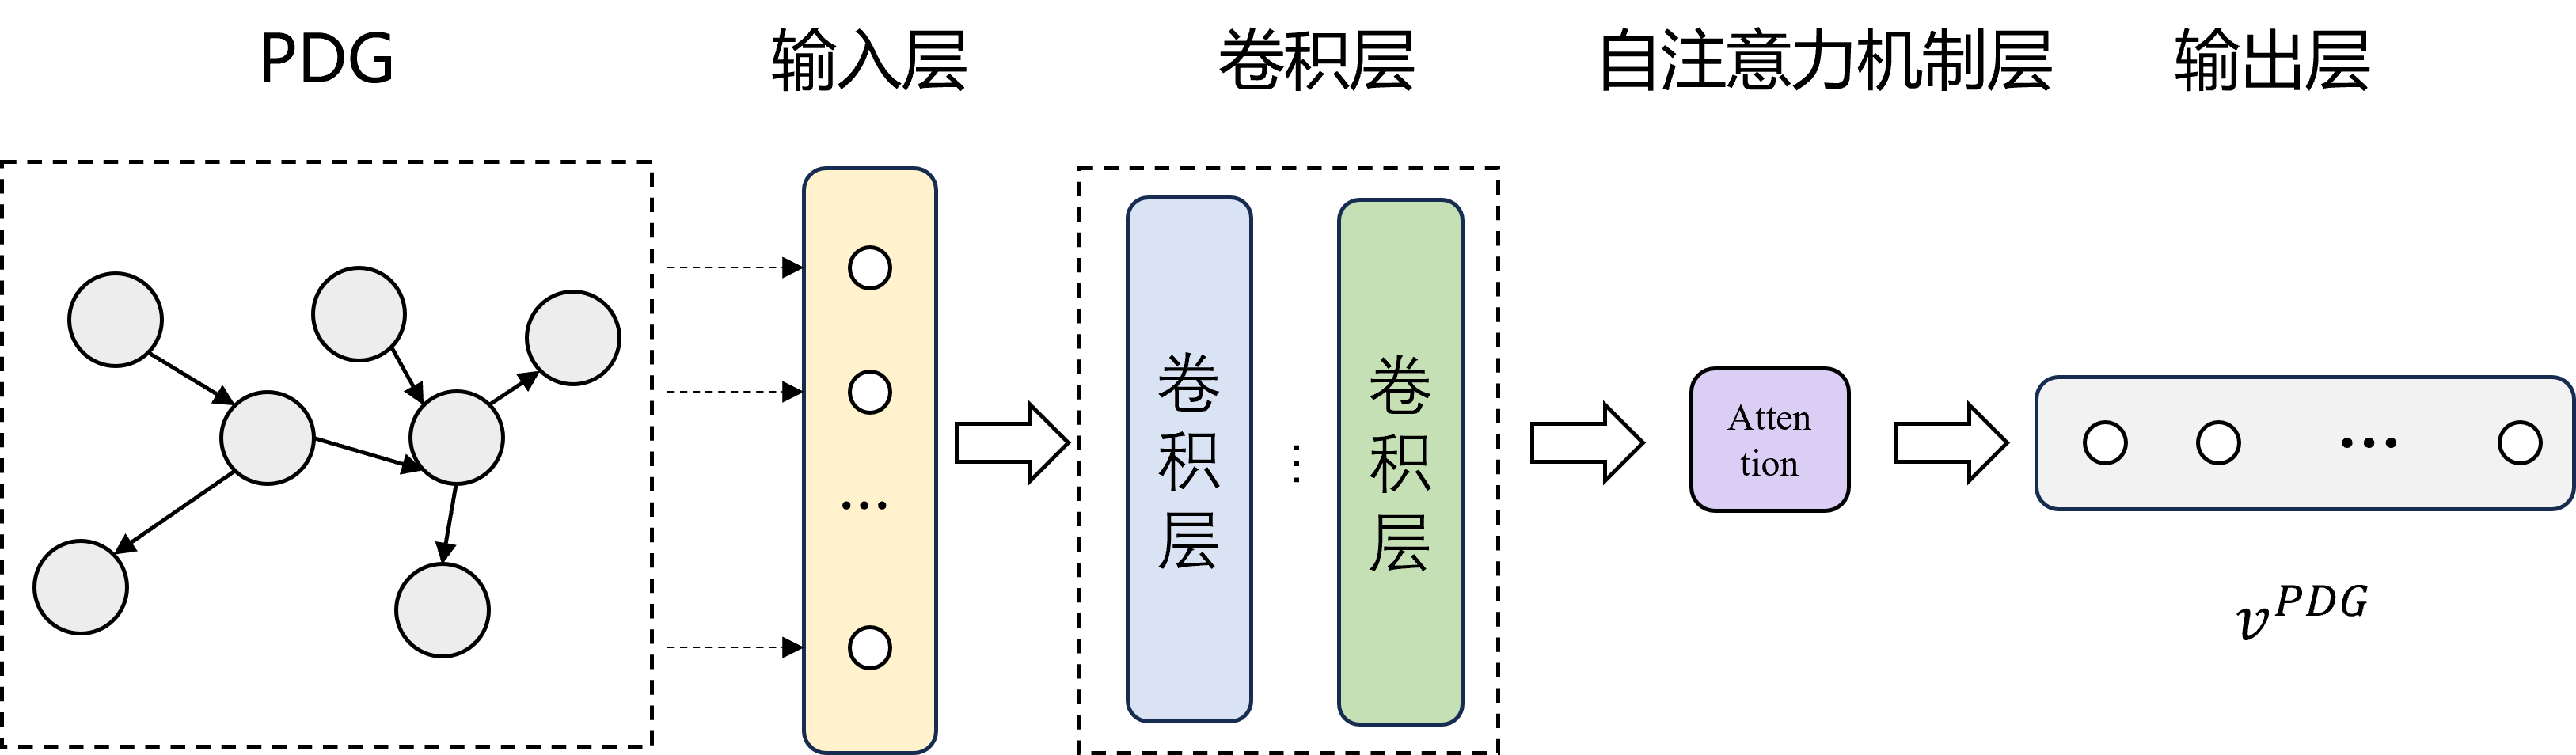
\includegraphics[width=0.85\textwidth]{figures/pdgmodel.png}
  \caption{程序依赖图表征模型设计}\label{fig:pdgmodel}
\end{figure}

\ding{172}输入层:输入层用于向模型输入训练数据,在本方法中模型的输入为经过过滤算法判断得到的程序依赖图。\ding{173}卷积层:由多层卷积层堆叠构成,通过卷积操作提取节点的特征,同时考虑到节点之间的关联。\ding{174}自注意力机制层:本层的主要目的是捕捉序列中的长距离依赖关系,通过直接计算任意两个位置的依赖关系,并将每个代码片段缩减为一个单一的密集向量。\ding{175}输出层:每个程序依赖图对应一个输出。

(2)模型选型

传统卷积神经网络中的卷积操作,是指利用滑动窗口在输入数据上平移,每次计算窗口内数据的有用特征,从而达到特征提取的目的。然而,这种操作只能处理图片、语言等结构规则的数据。现实中,像图结构这种不规则的数据普遍存在,其每个节点都拥有独特的邻接环境,无法通过传统CNN、RNN的方法计算。因此,有研究\cite{kipf2017semisupervised}提出图卷积神经网络。

在图结构中,每个节点都受到其邻居节点的影响,这种影响随着关系的紧密程度而变化,最终使节点达到稳定状态。图卷积神经网络(GCN)正是基于这样的思想,通过卷积操作来提取图中节点的特征。在GCN中,每个节点的特征表示不仅包含其自身的特征信息,还会考虑其所有邻居的特征信息,并通过学习得到的参数来更新。通过多层GCN的堆叠,可以逐步传播全局信息,实现对整个图的信息聚合和表示学习。相较于表真的CNN ,GCN能够很好地处理不规则和非欧氏空间的数据,因此在社交网络、化学分子结构、交通网络等领域有广泛应用。值得一提的是,图卷积操作具有置换不变性,即不依赖于节点的具体排序,这符合图数据的本质特性。

图卷积神经网络是一种特殊的前馈神经网络结构,为减少网络中参数个数,用卷积层来代替传统的全连接层,提高神经网络的训练效率,卷积神经网络可以提取信息最多的数据特征,生成一个固定大小的向量表示结构。这样的设计有助于深入挖掘数据的语法和语义信息,使得图卷积神经网络在代码克隆检测等任务中表现出色。

因此,本文选用图卷积神经网络来构建程序依赖图的表征学习模型,该模型通过聚合节点自身的信息和邻居节点的信息,实现节点表示的更新,通过多层图卷积堆叠,实现全图信息聚合,进而提升程序依赖图的特征提取能力。

首先给出GCN的符号定义:对于图$G=\left(V,E\right)$,其中$V$表示节点集,节点个数为$N$,对于每个节点$v_i \in V$,均有其特征向量$x_i$,节点的特征向量特征用矩阵$X \in R^{N×C}$表示,其中$C$表示每个特征向量的维度;$E$表示边的集合,如果节点$v_i$和$v_j$之间存在边,那么$\left(v_i,v_j\right) \in E$表示。在卷积过程中涉及到三种矩阵表示,因此本文给出下图\ref{fig:graph}示例。

\begin{figure}[H]
  \centering
  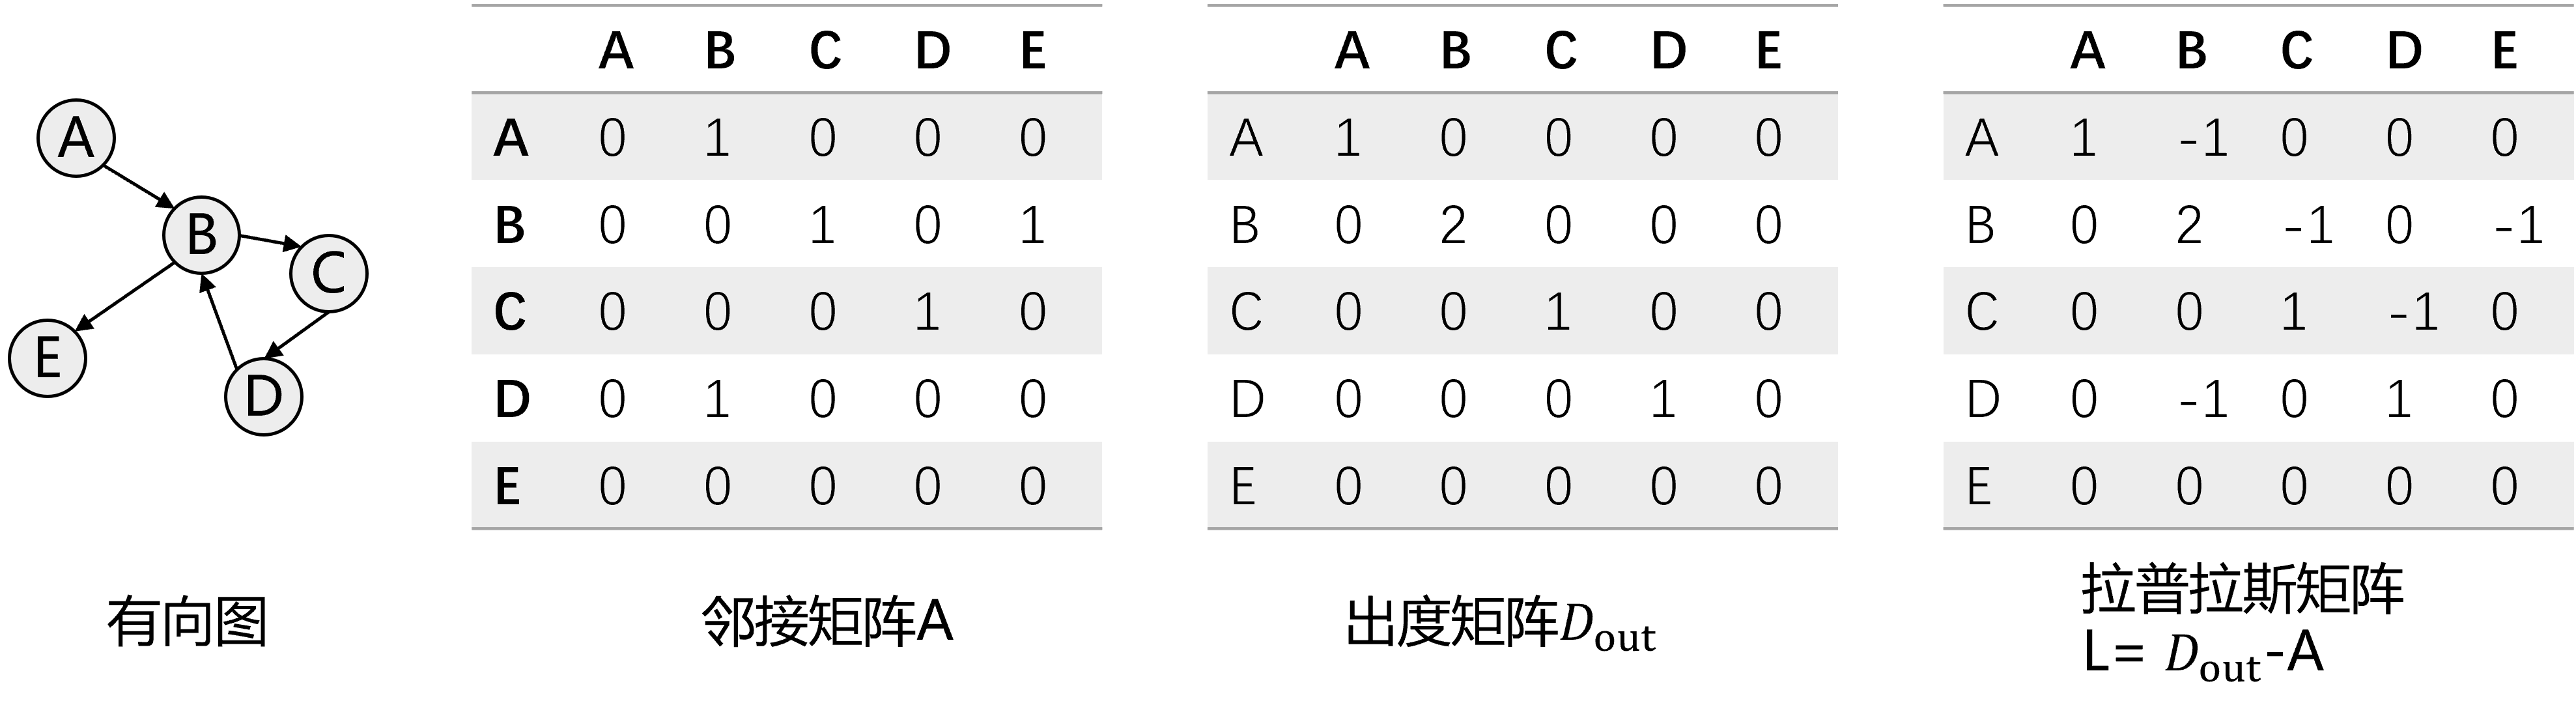
\includegraphics[width=0.95\textwidth]{figures/graph.png}
  \caption{有向图矩阵示例}\label{fig:graph}
\end{figure}

(1)邻接矩阵$A \in R^{N×N}$:用来表示图中节点之间关系的一种矩阵表示方法,如果存在从节点$v_i$指向节点$v_j$的边,那么$A[i][j] = 1$,如果不存在边,则$A[i][j] = 0$。(2)度矩阵$D \in R^{N×N}$:对角矩阵,用于表示图中每个节点的度(即与该节点相连的边的数量)。出度是从该节点出发的边的数量,入度是指向该节点的边的数量。度矩阵只有对角线上有值,对于节点$v_i$有$D[i][i] = \sum_j A_{ij}$,其他位置的元素都是0。对于有向图,可以分别构建入度矩阵$D_{in}$和出度矩阵$D_{out}$。(3)拉普拉斯矩阵$L \in R^{N×N} = D_{out} - A$:通过矩阵的形式描述了图的拓扑结构和性质,在图的传播和扩散问题中起到关键作用,通过特征值分解得到图的特征向量,有助于图的划分和聚类。

通过引入邻接矩阵和度矩阵,图卷积神经网络能够捕获图的拓扑结构信息,这是处理图数据的关键。该模型的输入$X \in R^{N×C}$为节点特征矩阵、$A \in R^{N×N}$为邻接矩阵,输出是一个特征矩阵$Z \in R^{N×F}$,表示学习到的每个节点的特征表示,$F$为模型自己定义的输出向量维度。下图\ref{fig:gcn}为图卷积神经网络结构图。
\begin{figure}[H]
  \centering
  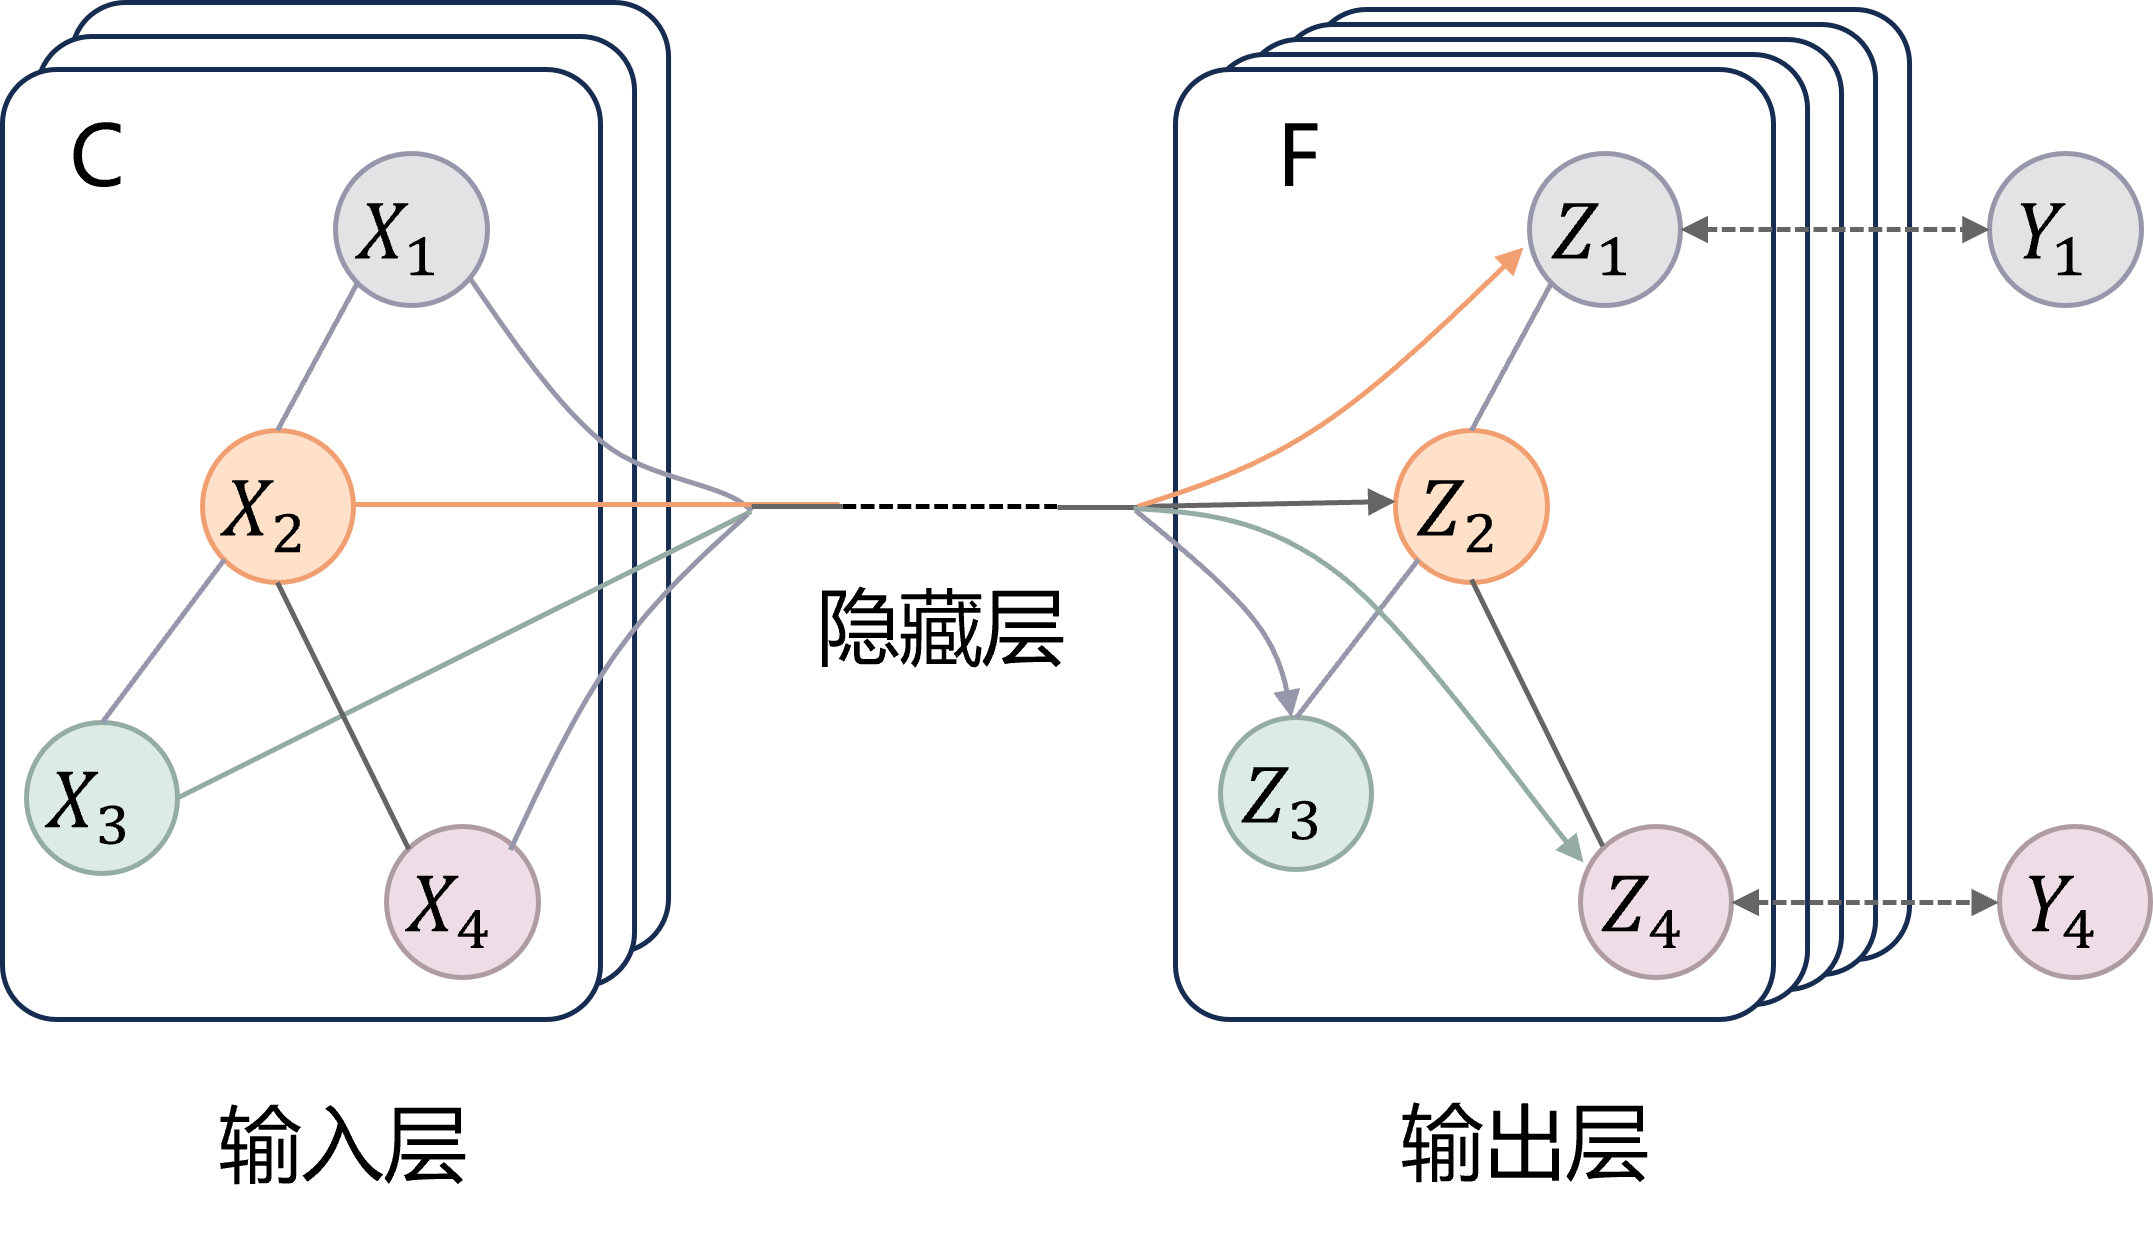
\includegraphics[width=0.55\textwidth]{figures/gcn.png}
  \caption{图卷积神经网络结构图}\label{fig:gcn}
\end{figure}

中间每一个图卷积层的输入都是邻接矩阵A和节点特征X,层与层之间的传播公式都可以写成\ref{e5.2};

\begin{equation}\label{e5.2}
  \begin{split}
    X^{l+1} = \sigma(\tilde{D}^{-\frac{1}{2}}\tilde{A}\tilde{D}^{-\frac{1}{2}}X^{l}W^{l})
  \end{split}
\end{equation}

其中:$X^{l}$ 表示第$l$层的节点特征矩阵。$W^{l}$是第 $l$层的参数,即可学习的权重矩阵。$\sigma$是激活函数,如ReLU。$\tilde{A} = A + I$,其中$I$是单位矩阵,表示给每个节点添加一条到自身的边,聚合时可以结合自身的特征消息。$\tilde{D}$是$\tilde{A}$的度矩阵,其公式为$\tilde{D[i][i]} = \sum_j \tilde{A_{ij}}$。对邻接矩阵$\tilde{A}$进行归一化操作$\tilde{D}^{-\frac{1}{2}}\tilde{A}\tilde{D}^{-\frac{1}{2}}$是为了信息传递的过程中保持特征矩阵$X$的原有分布,那些具有较低度的节点会对其邻居有较大的影响,而具有高度的节点会产生更小的影响因为他们的影响会被分散给很多的邻居节点。

\section{PDG表征方法具体实现}
\label{sec:PDGachieve}
在介绍具体实现之前,本节首先给出PDG表征方法的输入:经过\ref{subsec:Preprocess}小节的代码预处理阶段,得到示例代码片段\ref{fig:code}对应的程序依赖图,如图\ref{fig:pdgcode}所示。图中的实线表示节点之间的控制依赖,虚线表示节点之间的数据依赖。仔细分析三张图,其中图\ref{fig:pdg1}和图\ref{fig:pdg2}红框中节点11、12虽然位置有所改变,但是其边依赖均相同,因此可以视为完全相同的同构图;而图\ref{fig:pdg3}因为增加了一个if语句,图中也增加了一个节点,同时添加的红色的线表示新增的数据依赖、控制依赖。

\begin{figure}[htbp]
  \centering  %居中
  \subfigure[C语言代码片段1对应的PDG]{   %第一张子图
      \centering    %子图居中
      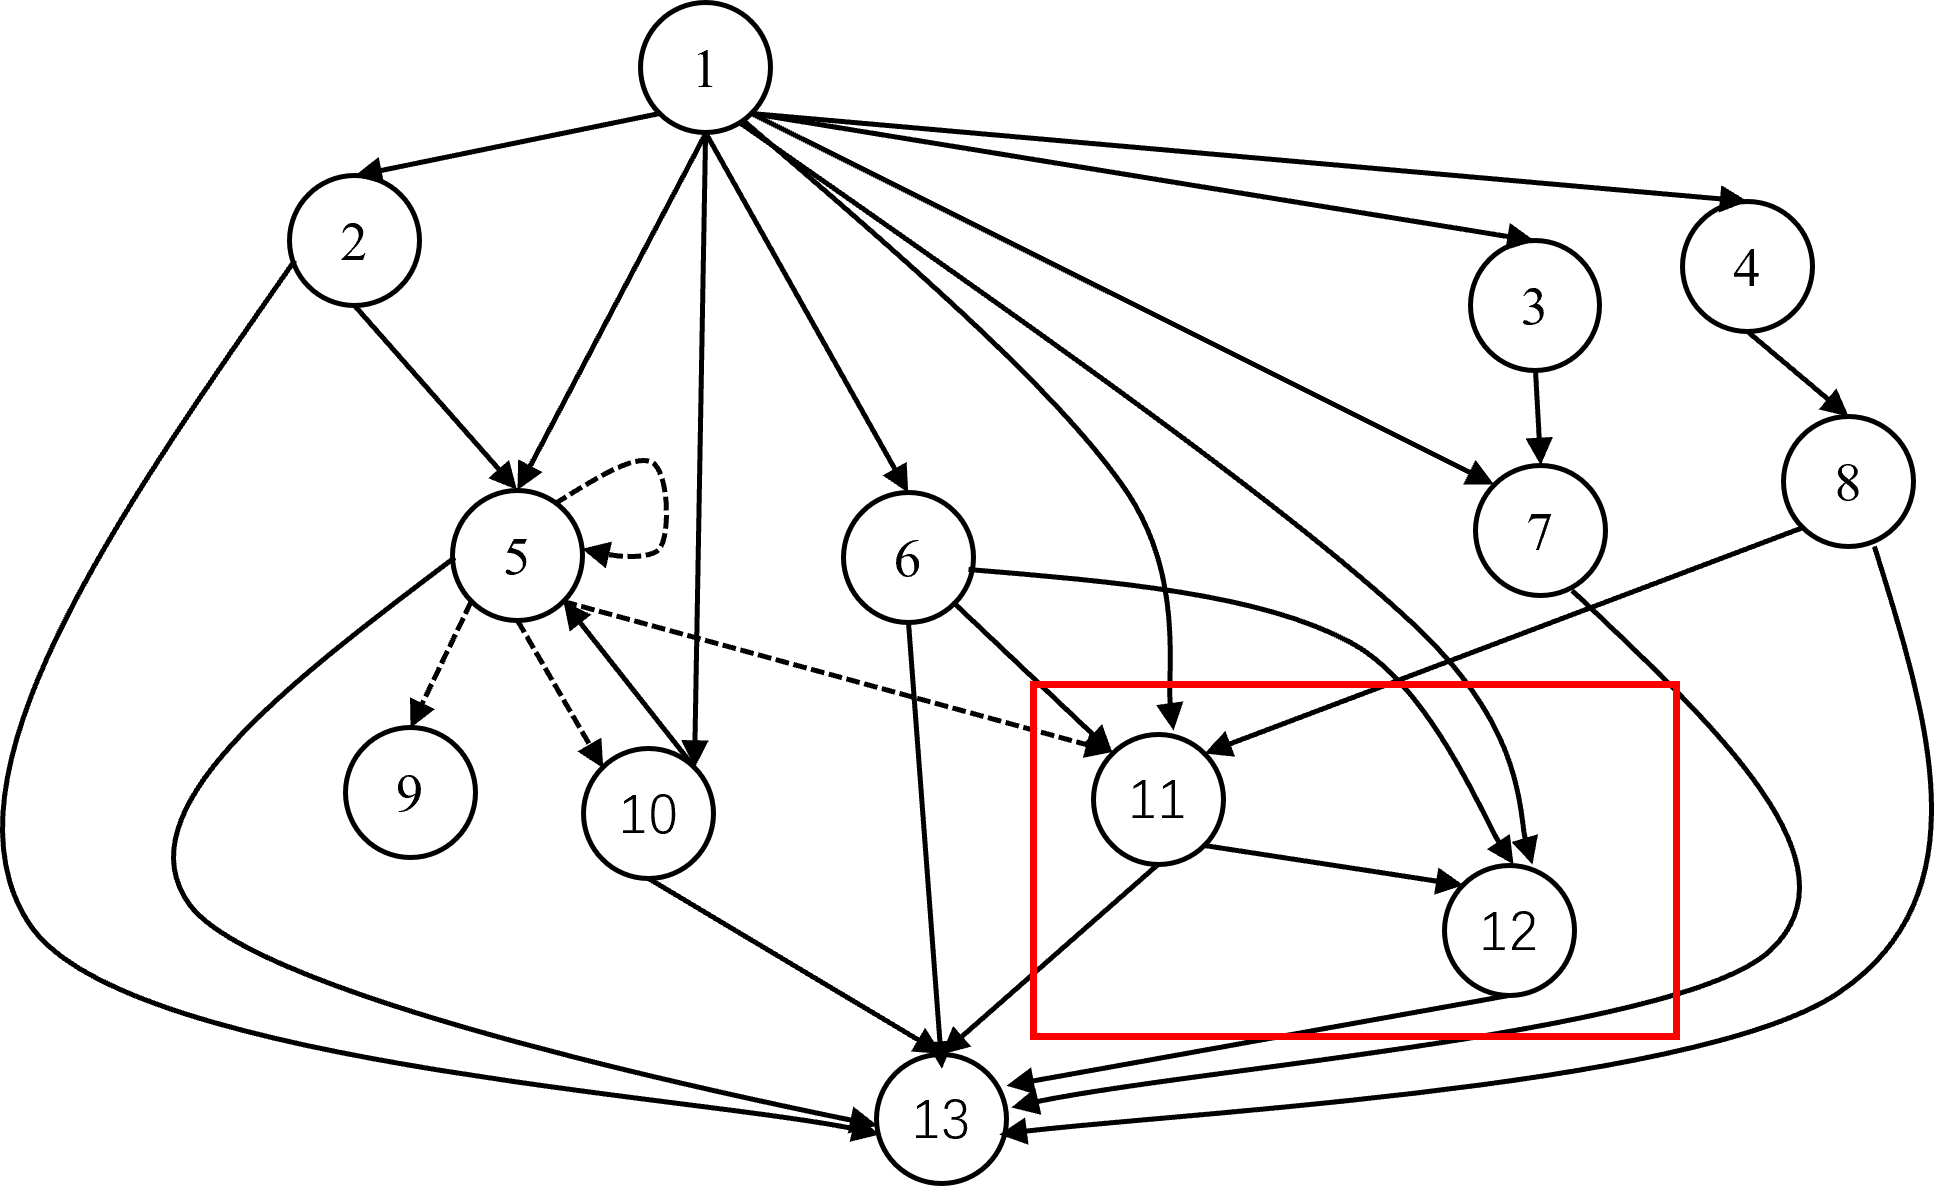
\includegraphics[width=0.3\textwidth]{figures/pdg1}  
      \label{fig:pdg1} %引用标签
  }
  \subfigure[C语言代码片段2对应的PDG]{ %第二张子图
      \centering    %子图居中
      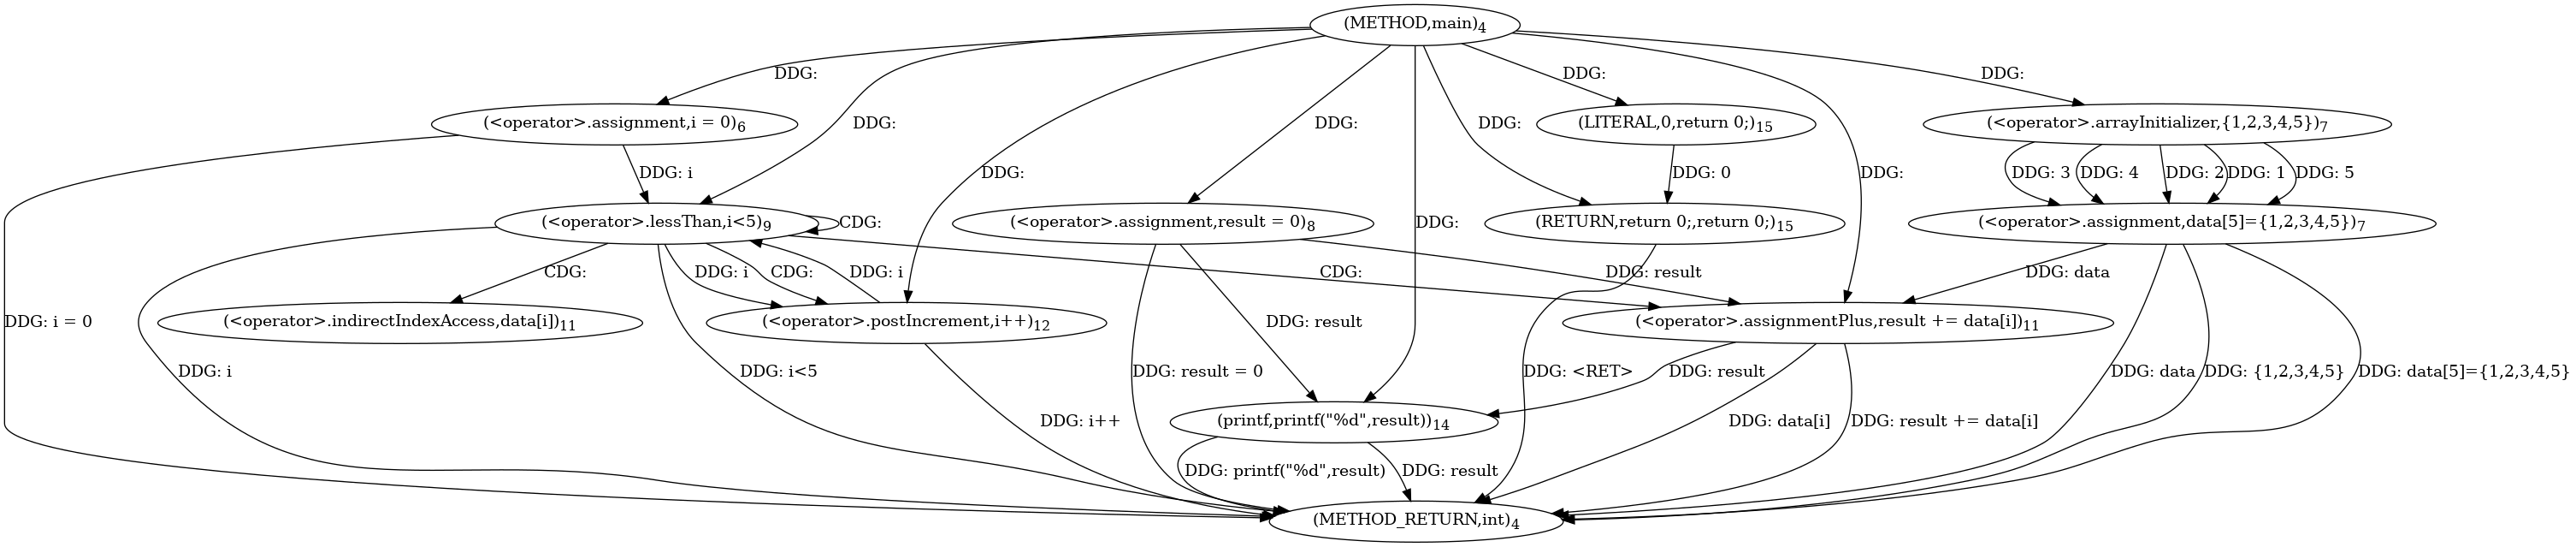
\includegraphics[width=0.3\textwidth]{figures/pdg2}
      \label{fig:pdg2} %引用标签
  }\subfigure[C语言代码片段3对应的PDG]{ %第二张子图
  \centering    %子图居中
  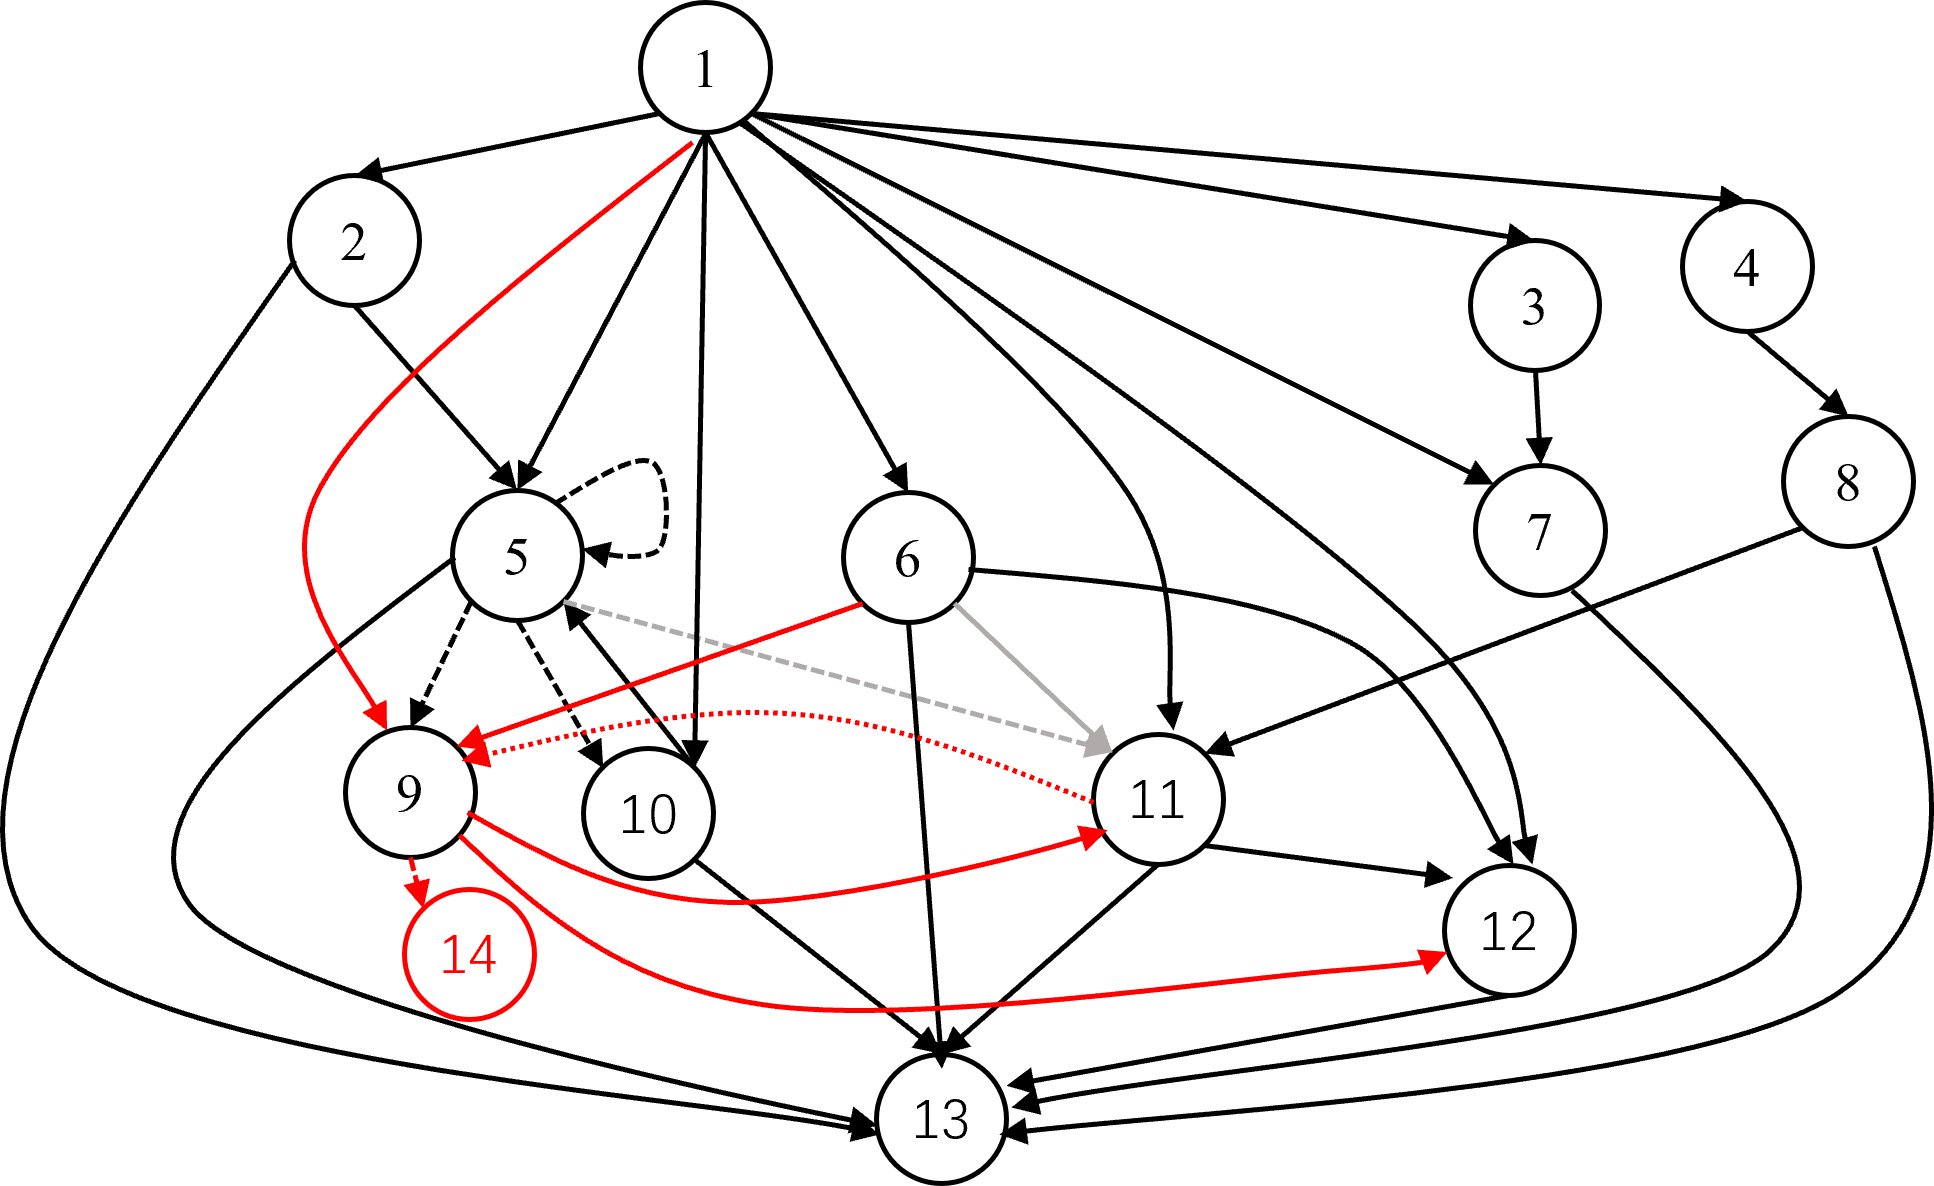
\includegraphics[width=0.3\textwidth]{figures/pdg3}
  \label{fig:pdg3} %引用标签
}
  \caption{示例源代码对应的程序依赖图}    %大图名称
  \label{fig:pdgcode}    %图片引用标记
\end{figure}

接下来,本章提出的基于图过滤的程序依赖图表征学习方法的实现如图\ref{fig:pdg}所示。该方法的输入是一对代码片段$C_{a},C_{b}$对应的程序依赖图,表示为$PDG_{a},PDG_{b}$,输出是$C_{a},C_{b}$对应的语义特征向量 $V_{a}^{PDG},V_{b}^{PDG}$,整体采用Siamese架构,两个子网络共享权值,从下到上,主要包括图过滤判断、图表征三个阶段。

\begin{figure}[H]
  \centering
  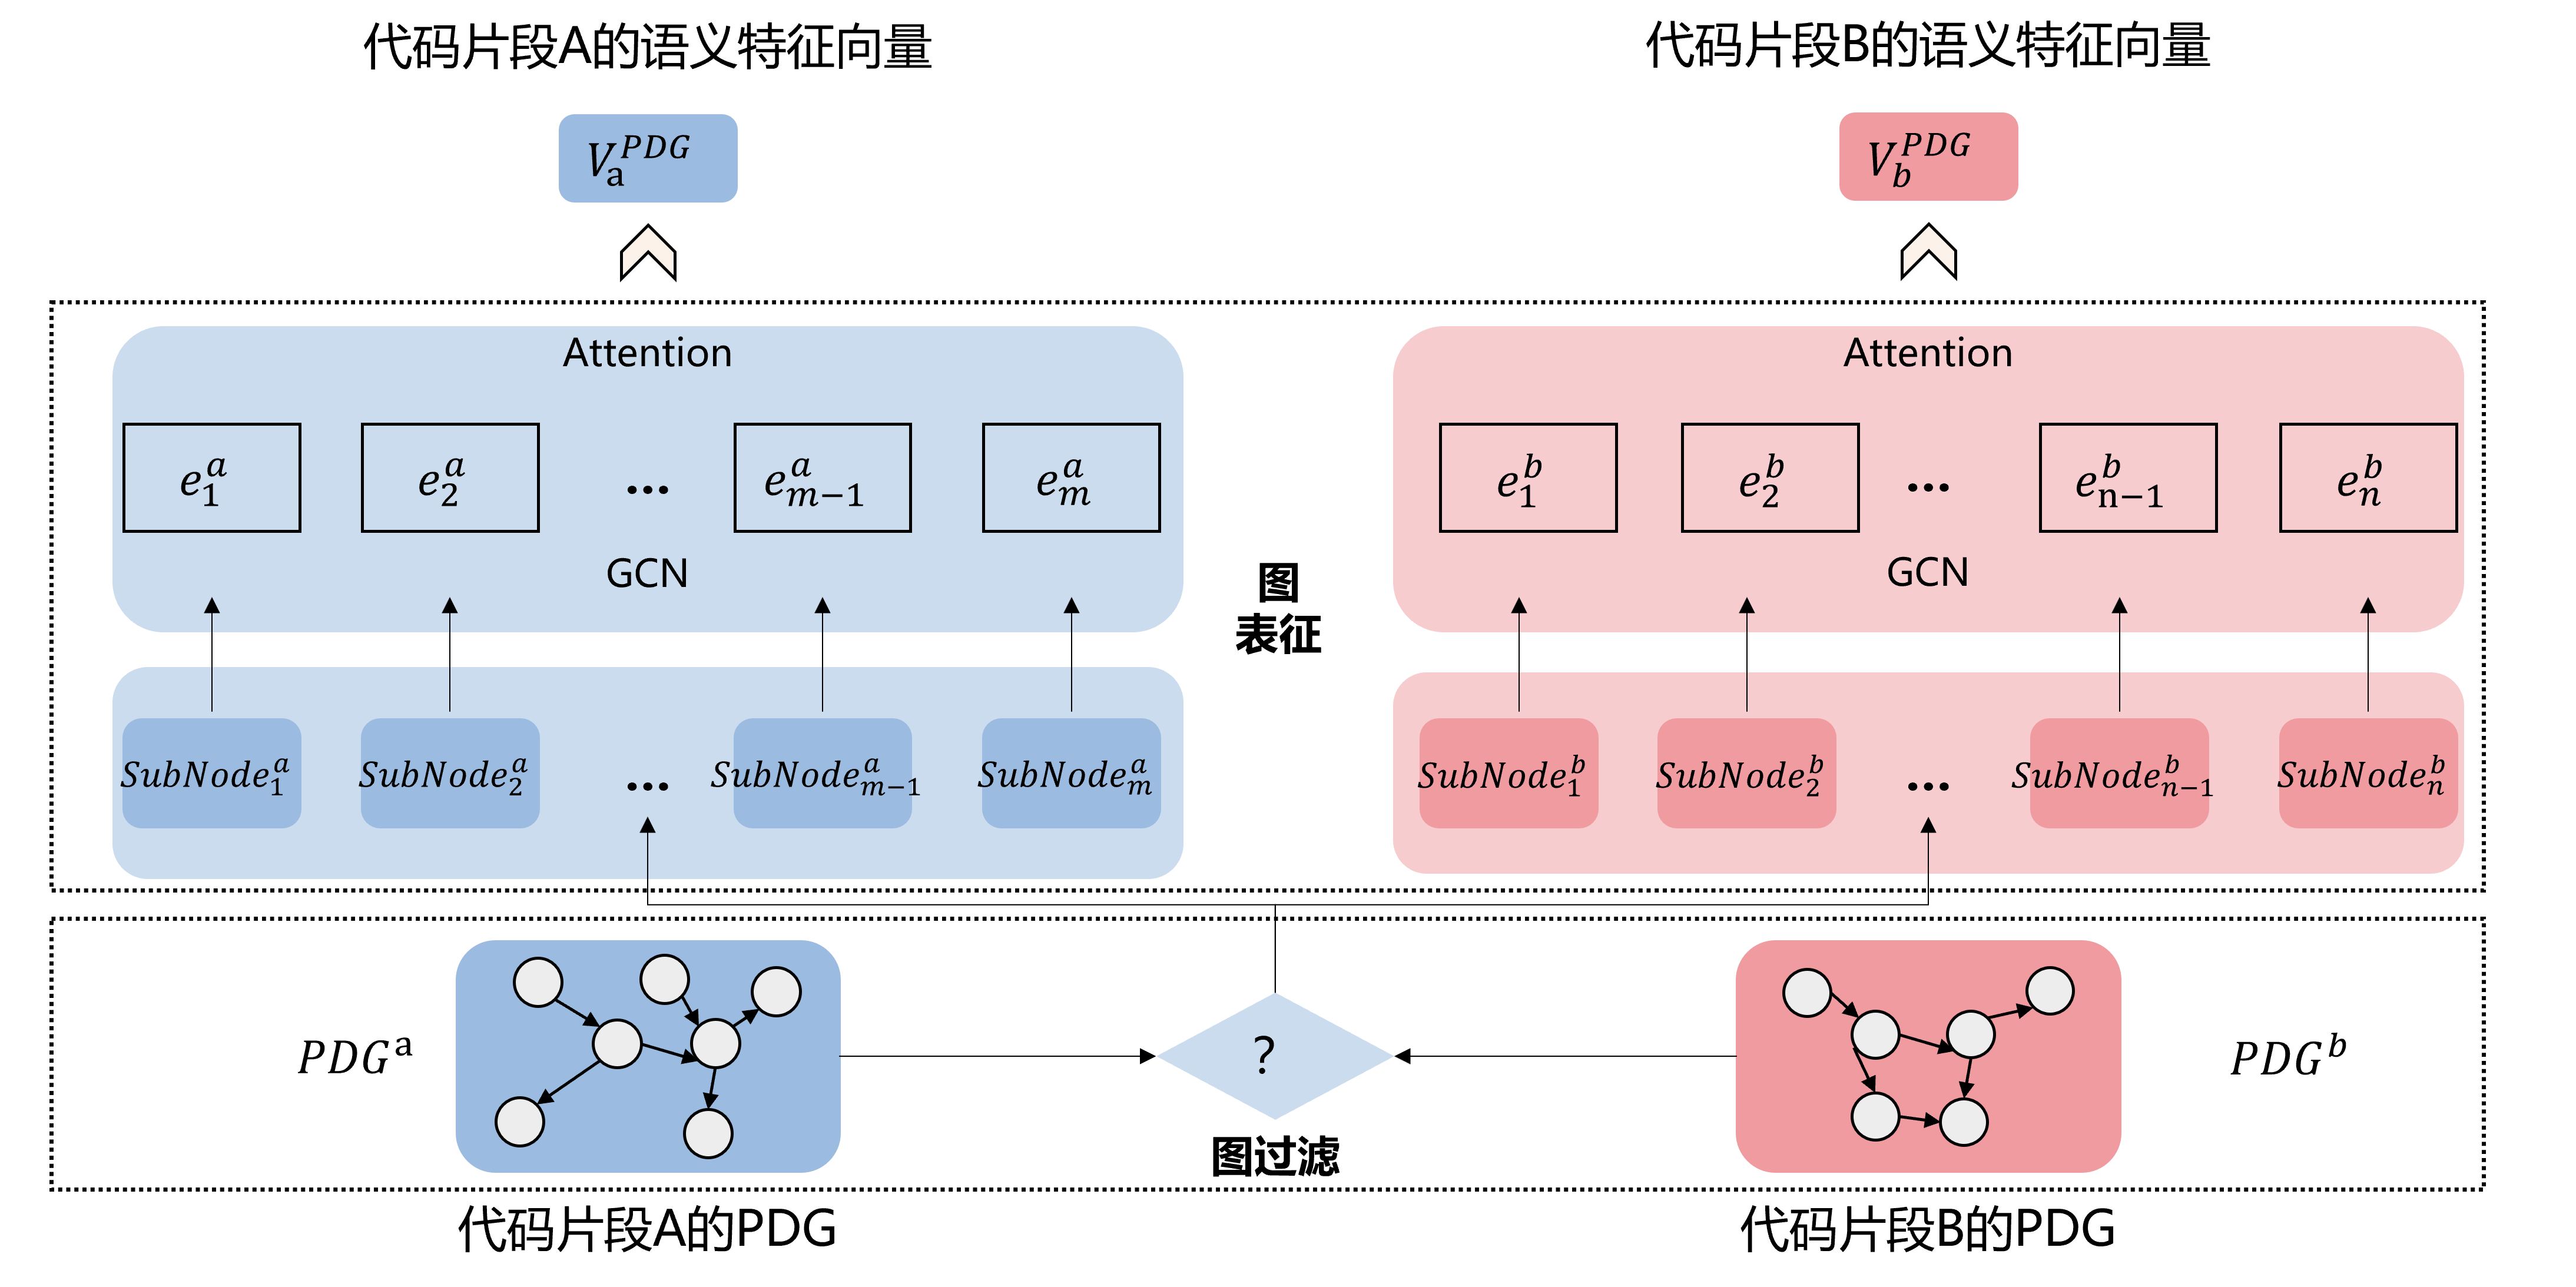
\includegraphics[width=0.9\textwidth]{figures/pdg.png}
  \caption{基于图过滤的程序依赖图表征学习方法实现}\label{fig:pdg}
\end{figure}

在图过滤阶段,将输入的PDG对进行过滤判定。首先对程序依赖图进行图结构约简,然后判断其有效行数是否大于6,是否存在子图同构,最后再判断两者的数值特征相似度是否大于阈值。如果顺利上述四个步骤,则该PDG对输入图表征模型。其过滤过程可以表达为公式\ref{e5.3}:

\begin{equation}\label{e5.3}
  \begin{split}
    \left(x_{1}^{a},x_{2}^{a},\ldots,x_{m}^{a}\right) = filter\_PDG \left(PDG_{a}\right)
  \end{split}
\end{equation}


在图表征模型,将PDG图作为输入,使用图卷积神经网络进行编码。处理过程分为两个步骤,如公式\ref{e5.4}所示。
\begin{equation}\label{e5.4}
  \begin{split}
    e_{1}^{aGCN},e_{2}^{aGCN},\ldots,e_{n}^{aGCN} = GCN\left(x_{1}^{a},x_{2}^{a},\ldots,x_{m}^{a}\right) \\
    V_{a}^{PDG} = Attention \left( e_{1}^{aGCN},e_{2}^{aGCN},\ldots,e_{n}^{aGCN} \right)
  \end{split}
\end{equation}

经过图卷积编码后,生成了$e_{i}^{aGCN}$,然后经过Attention层的总结后,生成了$V_{a}^{PDG}$作为代码片段$C_{a}$的最终图表示,即语义特征向量。
同样,可以使用相同的计算以通过图过滤判断的PDG作为输入为代码片段$C_{b}$计算$V_{b}^{PDG}$。

\section{实验验证}
\label{sec:PDGExperiment}
为了验证基于图过滤的程序依赖图表征学习方法的有效性,本节开展实验验证。首先,介绍了实验的具体设计,接着对子树划分、树表征模型进行消融实验。

\subsection{实验设计}
\label{sec:PDGDesign}

本节使用与\ref{sec:TokenExperiment}节中同样的实验环境、数据集对基于图过滤的程序依赖图表征学习方法进行对比实验。使用代码分析工具Joern获取数据集中代码片段的程序依赖图,然后使用图卷积神经网络训练图嵌入,并将嵌入向量大小设置为128。同样选取常用的精确率(Precision)、召回率(Recall)、F1值作为评估指标。

\subsection{实验结果}
\label{subsec:PDGResult}

(1) 图过滤机制的实验结果

为了探究图过滤机制对程序依赖图表征实验结果的影响,本文针对图过滤阶段中的:规模过滤、数值特征过滤两种策略进行了实验验证。其中,将规模过滤用PDG-size表示,数值特征过滤用PDG-Number表示,两种过滤策略均使用用PDG-All表示。本实验采取单一变量原则,仅修改图过滤策略,后续程序依赖图的编码采用相同的图卷积神经网络。具体实验结果如表\ref{tab:graph}所示。

\begin{table}[htp]
  \centering
  \caption{图过滤机制对实验结果的影响} 
  \label{tab:graph}
  \begin{tabular*}{0.9\textwidth}{@{\extracolsep{\fill}}ccccc}
  \toprule
   \multirow{2}{*}{图过滤策略} & \multirow{2}{*}{过滤后剩余PDG对} & \multicolumn{3}{c}{POJ104} \\
  \cmidrule{3-5} 
   & & 准确率P(\%) & 召回率R(\%) & F1值(\%)  \\ 
  \midrule
    PDG-Size		   & 6072	  &87.63	 &88.75		&88.19 \\
    PDG-Number		 & 7952	  &85.32   &82.65   &83.96 \\
    PDG-All		     & 5000	  &89.53   &81.71	 &85.44 \\
  \bottomrule
  \end{tabular*}
\end{table}

从表\ref{tab:graph}可以看出,本文使用的图过滤机制可以过滤掉大多数的候选PDG对。初始PDG对总数目为50000,经过过滤后的PDG对占原来PDG对数的比例大致在15\%以下,这意味着图过滤机制可以排除大部分候选PDG对,大大减少后续图表征模型的工作负担。同时面向代码克隆检测任务,不同PDG过滤策略处理后,其准确率、召回率、F1值相差不大,深究其原因,可能是在相似的图规模作为输入的情况下,图卷积模型训练策略没有差异,其代码信息表征能力也没有很大差异。因此,得出以下结论:本章提出的图过滤机制,面向代码克隆检测任务具有一定优势。考虑到后续输入图卷积神经网络的规模无需过大,避免给图表征模型带来过大训练压力,最终选择两种图过滤策略均使用的方法PDG-All作为图过滤机制。

(2) 图表征模型的实验结果

为了探究图表征模型对实验结果的影响,本文将图卷积神经网络与Weisfeiler-Lehman算法进行对比,结果如表\ref{tab:tree2}所示。其中Weisfeiler-Lehman(WL)算法是一种基于子图同构的检测算法,它的关键思想是通过对每个节点的所有相邻节点的标签排序,然后将标签根据某一映射压缩为新的更短的标签值来反映图中局部结构,通过统计两个图中相同标签值得数目判断两个图得相似度大小\cite{articleWL}。

其中,图卷积神经网络基于Pytorch1.10实现,其参数设置为:\ding{172} 图过滤:采用PDG-All的过滤方法。\ding{173} 表征模型的隐藏层维度设置为128,模型使用二元交叉熵作为损失函数,使用Adam优化器来训练模型参数,其中,学习率Learning\_rate设置为0.001,Dropout为0.5,训练批次Epochs为50,批处理大小Batch\_size为32,阈值Threshold为0.5,当相似度超过0.5,输入的代码对被判定为真克隆对,否则被判定为假克隆对。参数的确定是通过多次调试后选择最优参数作为最后的结果。\ding{174} WL算法对每个节点按照其类型进行数值化处理,采用(声明节点,赋值节点,控制节点,函数调用节点,其他节点)格式进行数值化。


\begin{table}[htp]  
  \centering  
  \caption{图表征模型对实验结果的影响}   
  \label{tab:graph2}
  %\renewcommand{\arraystretch}{1.1}  
  \begin{tabular*}{0.9\textwidth}{@{\extracolsep{\fill}}cccc}  
  \toprule  
  表征方法 & 准确率P(\%) & 召回率R(\%) & F1值(\%)  \\  
  \midrule
  Weisfeiler-Lehman图核算法  & 92.21	  & 52.13	 & 66.61		\\  
  图卷积神经网络		         & 89.53		&81.71		&85.44\\ 
  \bottomrule  
  \end{tabular*}  
\end{table}

基于对表\ref{tab:graph2}数据的分析,可以得到以下结论:(1)在对图进行表征的过程中,WL算法的准确率比图卷积神经网络更高。深究其原因,WL算法通过迭代更新节点的标签,可以捕获图的结构信息,算法实现简单,准确率高。(2)WL算法的召回率只有52.13\%。深究其原因,WL算法迭代过程中过于关注图结构信息,反而忽略了节点自身的特征信息,同时对迭代次数敏感,次数过少无法充分捕获图的结构信息。(3)综合F1值,图卷积神经网络对程序依赖图表征效果优势明显,面向代码克隆检测任务的实验结果更优秀。深究其原因,图卷积神经网络能够自动学习图节点的表示,同时聚合邻居节点的信息来更新节点的特征,从而捕获图结构信息、节点特征信息。因此,在图维度的代码表征模型选取上,本文更倾向于图卷积神经网络GCN。

(3)PDG表征可视化

为了更直观地展示本文提出的图过滤的PDG表征学习方法的有效性,本文使用t-SNE技术将高维Token维度属性特征向量可视化。按照预先设定的参数,图表征学习后生成的张量维度是128,本实验采用t-SNE技术将128维的张量转换为2维,得到的样本表征结果如图\ref{fig:pdgresult}所示。

\begin{figure}[H]
  \centering
  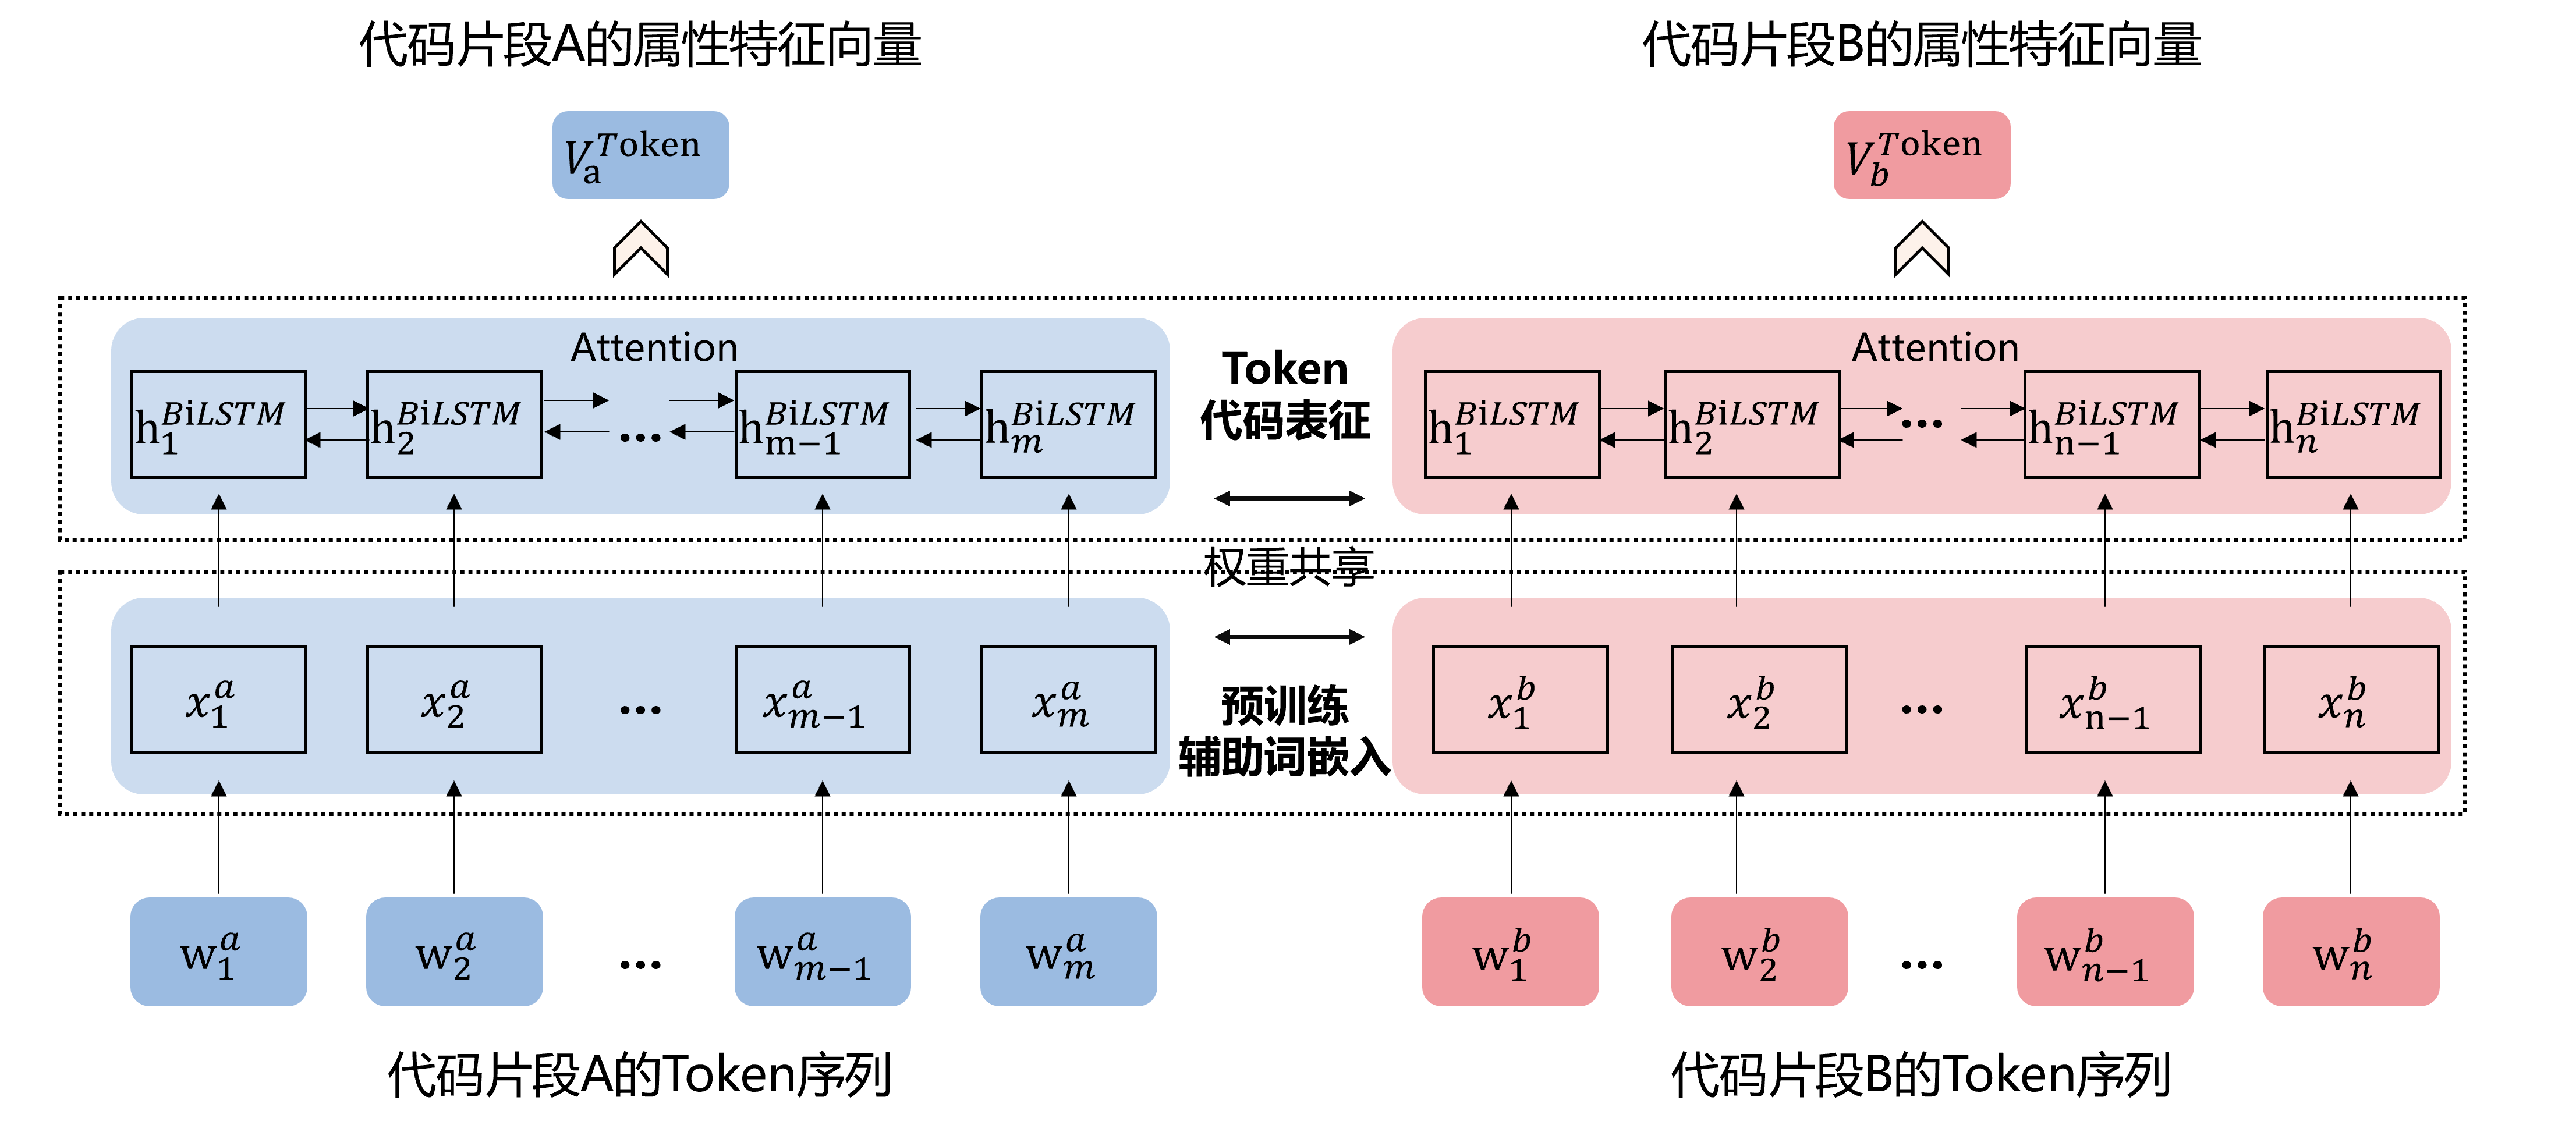
\includegraphics[width=0.9\textwidth]{figures/token}
  \caption{预训练辅助模型学习到的Token表征对比}\label{fig:pdgresult}
\end{figure}

分析上图,观察可视化结果,寻找可能的代码克隆群集。相似的代码片段在降维后的空间中应该更接近彼此。黑色代表label标签为1的样本,红色表示label标签为2的样本。经过训练,得到右图。

\section{本章小结}
\label{sec:Summary5}
本章主要对RLCCD中基于图过滤的程序依赖图表征学习方法的设计与实现进行详细阐述。首先介绍了程序依赖图维度的研究动机,其次介绍了程序依赖图表征学习的方法设计,具体论述了其整体框架、图过滤、图表征学习,接着开展实验验证,结果表明了此方法的有效性和模型的准确性。



